\documentclass[texcoord,
%    grid,
%    gridunit=mm,
%    gridcolor=red!60,
%    subgridcolor=gray!60,
    10pt]{beamer}
%\documentclass{beamer}
\usepackage[%
    texcoord,%
%    grid,%
%    gridunit=mm,%
%    gridcolor=red!60,%
%    subgridcolor=gray!60
]{eso-pic}
\usepackage{booktabs}
\usepackage[scale=2]{ccicons}
\usepackage{pgfplots}
\usepackage{xspace}
\usepackage[utf8]{inputenc}
\usepackage{graphicx}
\usepackage{pdflscape}
\usepackage{pdfpages}
\usepackage{verbatim}
%
\usepackage{xcolor}
\usepackage{times}
\usepackage{tikz}
\usepackage{caption}
\usepackage{subcaption}
\usepackage{float}
\usepackage{multirow}
\usepackage{multicol}
\usepackage{enumerate}
\usepackage{amsmath}
\usepackage{amssymb}
\usepackage{graphicx}
\usepackage{latexsym}
\usepackage{ucs}
\usepackage{siunitx}
\usepackage{times}
\usepackage{tikz}
\usepackage{verbatim}
\usepackage{pgf,pgfarrows,pgfnodes,pgfautomata,pgfheaps,pgfshade}
\usepackage{listings}
\usepackage{esint}
\usepackage{mathptmx}
\usepackage{helvet}
\usepackage{tikz}%
\usepackage{csvsimple}
\usepackage{pgfplots}
\usepackage{proba}
\usepackage[absolute, overlay]{textpos}
\usepackage{bibunits}
\usepackage{tcolorbox}
\usepackage{mathtools}
\usepackage{epigraph}
\setlength{\epigraphwidth}{.8\textwidth}
\usepackage{DejaVuSansMono}
\usepackage{svg}
\usepackage{qrcode}
\newcommand{\insertqrcode}{%
    \qrcode{https://github.com/SaulDiazInfante/Baemer-SIAM-Section-Mexico-third-annual-Metting}
}
%
\tolerance=1000
%\newcommand{\themename}{\textbf{\textsc{metropolis}}\xspace}
%\renewcommand{\raggedright}{\leftskip=0pt \rightskip=0pt plus 0cm}
%\newcommand{\jus}{\justifying}
%\apptocmd{\frame}{}{\justifying}{}
%\apptocmd{\block}{}{\justifying}{}
%\apptocmd{\column}{}{\justifying}{}
\hypersetup{colorlinks,citecolor=verde,linkcolor=orange,urlcolor=verde}
%=============================
\usetheme[sectionpage=none, subsectionpage=progressbar]{metropolis}
\usepgfplotslibrary{dateplot}
\useoutertheme[subsection=false,footline=authortitle]{miniframes}
\setbeamertemplate{footline}[frame number]%Numerando as Páginas
\hypersetup{pdfpagemode=FullScreen}%Visualizar em Tela cheia
\hypersetup{pdfpagelayout=SinglePage}%Layout da pagina
%\providecommand{\sin}{} \renewcommand{\sin}{\hspace{2pt}\textrm{sen}}
%\providecommand{\tan}{} \renewcommand{\tan}{\hspace{2pt}\textrm{tg}}
\setbeamerfont{section in toc}{size=\small}
\setbeamerfont{subsection in toc}{size=\scriptsize}%\footnotesize
\setbeamerfont{subsubsection in toc}{size=\scriptsize}
\AtBeginEnvironment{minted}{\renewcommand{\fcolorbox}[4][]{#4}}
\AtBeginSection[]{
    \begin{frame}<beamer>
        \frametitle{}
        \tableofcontents[currentsection]
    \end{frame}
}
\definecolor{verde}{HTML}{008069}
\definecolor{verdepastel}{HTML}{d8f3dc}
\definecolor{verdesolution}{HTML}{beff9e}
\definecolor{vsplbggray}{HTML}{f4f8ff}
% %-----------------------------------------------
\setbeamercolor{alerted text}{fg=orange}
\setbeamercolor*{palette primary}{fg=verde!60!black,bg=gray!30!white}
\setbeamercolor*{palette tertiary}{bg=verde!90,fg=white}
\setbeamercolor*{palette quaternary}{fg=verde,bg=gray!5!white}
\setbeamercolor*{sidebar}{fg=black,bg=black}
\setbeamercolor{progress bar}{fg=verde}%Linha q passa as seções
\setbeamercolor*{titlelike}{parent=palette primary}
\setbeamercolor{titlelike}{parent=palette primary,fg=verde}
\setbeamercolor{frametitle}{bg=verdepastel,fg=verde}
\setbeamercolor{frametitle right}{bg=black}
\setbeamercolor{background canvas}{bg=white}
%
\setbeamertemplate{blocks}[rounded][shadow]
%
\definecolor{vblock}{HTML}{E30022}
\BeforeBeginEnvironment{problem}{
\setbeamercolor{block title}{fg=vblock,bg=red!30!white}
\setbeamercolor{block body}{fg=vblock, bg=red!15!white}
}
\AfterEndEnvironment{problem}{
\setbeamertemplate{itemize subitems}[circle]
\setbeamercolor{blocktitle}{
    use=structure,fg=structure.fg,bg=structure.fg!20!bg
}
\setbeamercolor{block body}{
    parent=normal text,use=block title,bg=block
    title.bg!50!bg, fg=black}
}
%
\BeforeBeginEnvironment{solution}{%
    \setbeamercolor{block title}{fg=verde,bg=verdesolution}
    \setbeamercolor{block body}{fg=verde, bg=green!5!white}
}
\AfterEndEnvironment{solution}{
 \setbeamercolor{block title}{
    use=structure,
    fg=structure.fg,
    bg=structure.fg!20!bg
}
    \setbeamercolor{block body}{
        parent=normal text,
        use=block title,
        bg=blocktitle.bg!50!bg,
        fg=black
    }
}
\setbeamercolor{block title example}{
    use=example text,
    fg=example text.fg,
    bg=example text.fg!50!bg
}
\setbeamercolor{block body example}{
    parent=normal text,
    use=block title example,
    bg=block title example.bg!50!bg
}
\tcbuselibrary{skins, breakable}
%
\newtcolorbox{greenbox}[1]{%
        colback = green!5!white,
        colframe = green!55!black,
        fonttitle = \bfseries,
        title = #1
}
\newtcolorbox{bluebox}[1]{%
        colback = blue!5!white,
        colframe = blue!55!black,
        fonttitle = \bfseries,
        title = #1
}
%
\newtcolorbox{graybox}[1]{%
        colback = gray!5!white,
        colframe = gray!55!black,
        fonttitle = \bfseries,
        title = #1
}
%
\newtcolorbox{yellowbox}[1]{%
        colback = yellow!5!white,
        colframe = yellow!55!black,
        fonttitle = \bfseries,
        title = #1
}
\graphicspath{{./images}}

%
\title{Uncertainty quantification of vaccination policies:
}%
    \subtitle{%
        \textcolor{orange}{%
            a model for stock management with random fluctuations.
        }
    }
    \date{\textcolor{brown}{June 9,  2022}}
    \author{\bf
        YHG, SDIV, AMS
    }
    \institute{
        \textcolor{verde}{
            UNACH,
            CONACYT-Universidad de Sonora,
            Universidad de Sonora
        }
    }
\titlegraphic{
    \begin{picture}(0,0)
        \put(330, 15){
             \makebox(0,0)[rt]{
                 %
\includegraphics[width=2.5cm]{./images/logo_siam.png}
                
\includegraphics[width=12.5cm]{./images/logo_header.png}
            }
        }
    \end{picture}
 }
\begin{document}
    \maketitle
     \section*{Introduction}
         \subsection{Motivation}
    \begin{frame}{Problem}
        As part of the COVID-19 vaccination campaing, on December 02
        2020, Mexican goverment anunciates a series of the ***
        vaccine deliveries by Pfizer-BioNtech.
        \begin{textblock*}{130mm}(1mm, 20mm)
        \only<1>{
            %\begin{bluebox}{Delivery schedule}
                \begin{center}
                    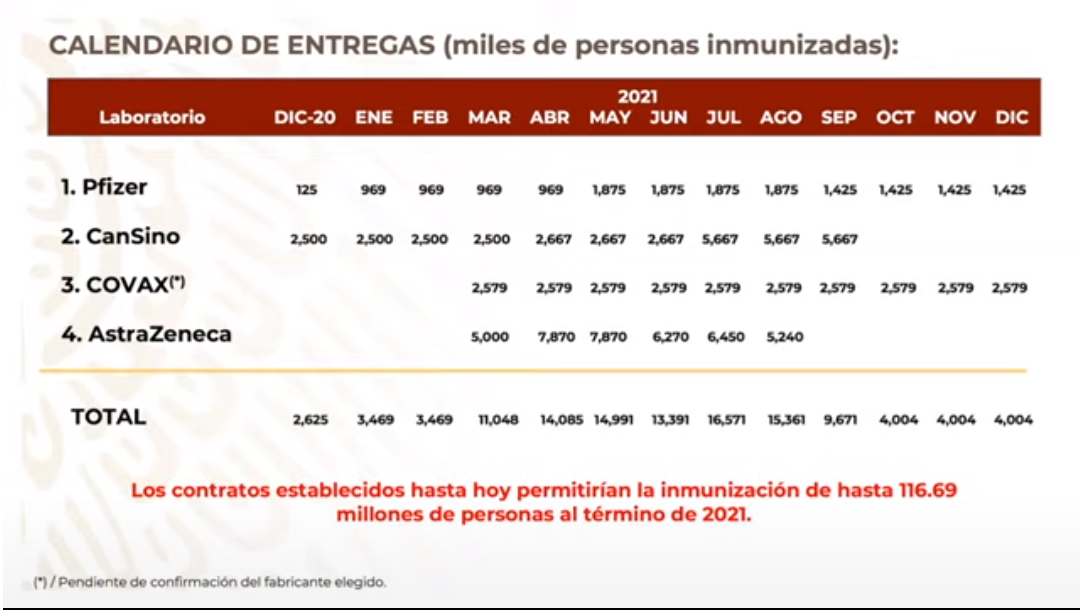
\includegraphics[%
                        width=\textwidth,
                        keepaspectratio=true]{screenshot.png}
                \end{center}
            %\end{bluebox}
        }
    \end{textblock*}
    \end{frame}
%
\begin{frame}{Argument}
    \begin{textblock*}{50mm}(10mm, 30.0mm)
            We argue that sufficiently large random fluctuations in
        deliveries\textemdash due to lags or the
        number of vaccines doses\textemdash convey significantly
        effects on the mitigation of
        symptomatic cases.
\end{textblock*}

    \begin{textblock*}{50mm}(70mm, 30.0mm)
    \begin{block}{Aims}
        We pursue quantifying the uncertainty due to time lags or amount
        delivery, and evaluates its implications.
    \end{block}
    \end{textblock*}
\end{frame}
%%%%
\subsection{Methodology}
    \begin{frame}{Methodology}
        Given a shipment of vaccines calendar, describe the stock management with
        backup protocol and quantify random fluctuations due to schedule or
        quantity. Then plug this dynamic with an ODE system that describes the
        disease and evaluates its response accordingly.
    \end{frame}
%
\begin{frame}{Vaccine Shipment Program}
    As part of the COVID-19 vaccination campaign, on December 02, 2020, the
    Mexican government annunciated a delivery plan of vaccines by Pfizer-BioNTech
    and other firms.
    \begin{textblock*}{130mm}(1mm, 20mm)
    \only<2>{
        %\begin{bluebox}{Delivery schedule}
            \begin{center}
                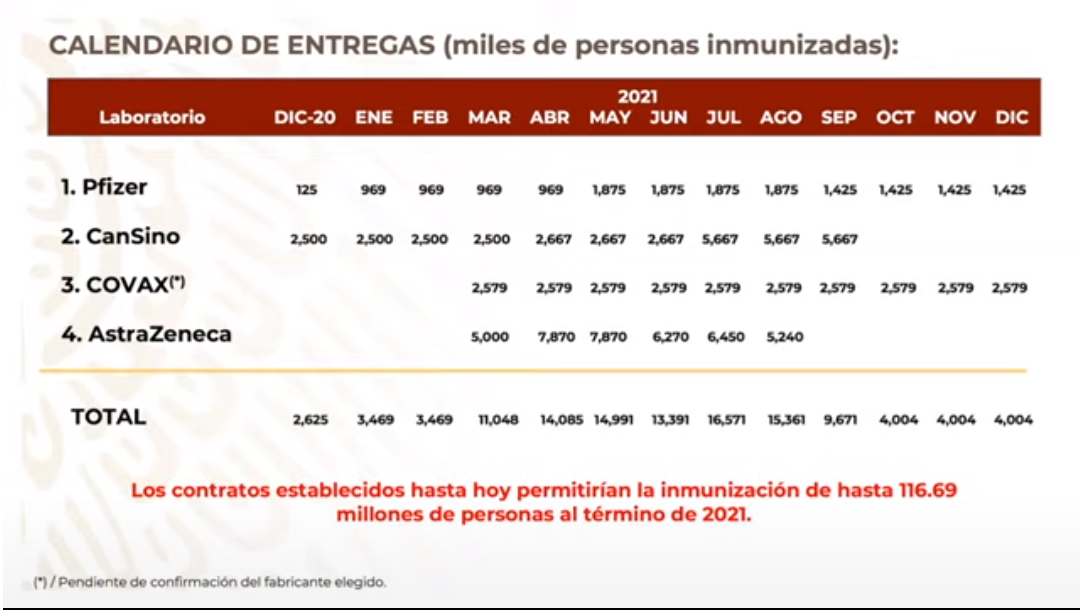
\includegraphics[%
                    width=\textwidth,
                    keepaspectratio=true]{screenshot.png}
            \end{center}
        %\end{bluebox}
        }
    \end{textblock*}
 \end{frame}



     \begin{frame}{Outline}
         \hypersetup{linkcolor=black}
         \setbeamertemplate{section in toc}[sections numbered]
         \tableofcontents
     \end{frame}
     \section{Model Formulation on continuous time}
         %!TEX root = ../main.tex
\begin{frame}{Toy example and classic vaccination OC}
    \setlength{\leftmargini}{1mm}
    \begin{textblock*}{65mm}(0mm, 18mm)
        \only<1->{
            To fix ideas:
            \begin{equation*}
                \begin{aligned}
                    S'(t) &= -\beta IS
                    \\
                    I'(t) &=  \beta IS - \gamma I
                    \\
                    R'(t) & = \gamma I
                    \\
                    & S(0) = S_0, I(0)=I_0, R(0)=0
                    \\
                    & S(t) + I(t) + R(t )= 1
                \end{aligned}
            \end{equation*}
        }
    \end{textblock*}
%     %
    \begin{textblock*}{65mm}(65mm, 18mm)
        \only<2>{
            With vaccination
            \begin{equation*}
                \begin{aligned}
                    S'(t) &= -\beta IS  - \textcolor{red}{\lambda_V(t)}
                    \\
                    I'(t) &=  \beta IS - \gamma I
                    \\
                    R'(t) & = \gamma I
                    \\
                    V'(t) & = \textcolor{red}{\lambda_V(t)}
                    \\
                    & S(0) = S_0, I(0)=I_0,
                    \\
                    &R(0)=0, V(0) = 0
                    \\
                    & S(t) + I(t) + R(t) + V(t)= 1
                \end{aligned}
            \end{equation*}
        }
    \end{textblock*}
    \begin{textblock*}{65mm}(65mm, 18mm)
        \only<3->{
            \begin{equation*}
                \begin{aligned}
                    S'(t) &= -\beta IS  - \textcolor{red}{\lambda_V(x, t)}
                    \\
                    I'(t) &=  \beta IS - \gamma I
                    \\
                    R'(t) & = \gamma I
                    \\
                    V'(t) & = \textcolor{red}{\lambda_V(x,t)}
                \end{aligned}
            \end{equation*}
        }
    \end{textblock*}
    \begin{textblock*}{28mm}(5mm, 50mm)
        \begin{block}{``Classic'' Vaccination}
            \begin{itemize}
                \item
                \only<4->{
                    Gumel,
                }
                \only<6->{
                    $$
                    \lambda_V:=
                    \underbrace{ \textcolor{orange}{\xi}}_{cte.}
                    \cdot \ S(t)
                    $$
                }

            \end{itemize}
            \only<7->{
                Optimal Controlled:
            }
        \end{block}
    \end{textblock*}
    \begin{textblock*}{80mm}(45mm,48mm)
            \only<6>{
                \begin{bibunit}[apalike]
                    \nocite{Alexander2004,Iboi2020}
                    \putbib
                \end{bibunit}
            }
            \only<7>{
                \begin{bibunit}[apalike]
                    \nocite{Hethcote1973,Wickwire1977}
                    \putbib
                \end{bibunit}
            }
    \end{textblock*}
 \end{frame}
% %%%%%%%%%%%%%%%%%%%%%%%%%%%%%%%%%%%%%%%%%%%%%%%%%%%%%%%%%%%%%%%%%%%%%%%%%%%%%%
\begin{frame}{The Basic Optimization Question}
    \begin{textblock*}{72.5mm}(0mm, 10mm)
        \begin{graybox}{Hypothesis}
            \only<1->{
                \textbf{Cost:}
                The \textbf{effort} expended in
                ``\textbf{preventing-mitigating}
                an epidemic'' by vaccination is
                \textbf{proportional} to the vaccination
                rate $\lambda_V$.\\
            }
%            %
            \only<2->{
                \textbf{Jabs Counter:}
                If $S(0)\approx 1$ , $X(\cdot):$ counts
                vaccine doses, then
                $$
                X(t) = 1 - \exp(-\lambda_V t),
                $$
                estimates the fraction of vaccinated
                individuals.
                Thus, for time horizon $T$ and
                vaccination coverage %$X_{cov}$
            }
            \only<3-6>{
                \begin{equation*}
                    \begin{aligned}
                        X_{cov} &= X(T)
                        \\
                        &\approx
                        1 - \exp(-\textcolor{teal}{\lambda_V} T).
                    \end{aligned}
                \end{equation*}
            }
        \end{graybox}
    \end{textblock*}
    \begin{textblock*}{50mm}(75mm, 10mm)
        \only<4->{
            \begin{yellowbox}{{Given $X_{cov}$, \ $T$}}
                $$
                \lambda_V = -\frac{1}{T}
                \ln(1 - X_{cov})
                $$
                \textbf{estimates} the constant vaccination rate s.t.,
                afther time $T$, we reach $X_{cov}$.
            \end{yellowbox}
        }
        \only<5->{
            \begin{greenbox}{{$X_{COV}: 70 \%$, $T$: one \SI{}{year}}}
                $
                \lambda_V \approx \num{0.00329}
                $
                \tcblower
                \only<6>{
                    If $S(0) N$ corresponds to HMS
                    (\SI{812229}{inhabitants})
                    $
                    % \num{0.00611352} \times \num{100000}
                    \approx \SI{2668}{jabs \per day}.
                    $
                }
                \only<7->{
                    \textcolor{orange}{
                        \textbf{
                            How to optimize vaccination?}
                    }
                }
            \end{greenbox}
        }
    \end{textblock*}
%     %--------------------------------------------------------------------------
    \setbeamertemplate{itemize items}[ball]
    \begin{textblock*}{62mm}(5mm, 70mm)
        \only<8->{
            \begin{block}{Common Objectives}
                \begin{itemize}
                    \item
                    \only<9->{

                        Who to vaccine first?
                        (Allocation)
                    }
                    \item
                    \only<10->{

                        How and when?
                        (Administration)
                    }
                \end{itemize}
            \end{block}
        }
    \end{textblock*}
\end{frame}
%%%%%%%%%%%%%%%%%%%%%%%%%%%%%%%%%%%%%%%%%%%%%%%%%%%%%%%%%%%%%%%%%%%%%%%%%%%%%%%%
 \begin{frame}{Vaccine optimiztion for COVID-19}
    \begin{textblock*}{40mm}(5mm, 15mm)
        \setbeamertemplate{itemize items}[ball]
        \begin{block}{Common Objectives}
             \begin{itemize}%
                 \item
                 \textcolor<5>{orange}{
                     Who to vaccine first?
                     (Allocation)
                 }
                 \only<2->{
                     \item
                     \textcolor<6->{orange}{
                         How and when?
                         \textbf<7>{
                             (Administration)
                         }
                     }
                 }
             \end{itemize}
         \end{block}
    \end{textblock*}
%     %
    \begin{textblock*}{65mm}(55mm, 15mm)
        \only<2->{
            \begin{block}{%
                    \only<2-3>{Cost}
                    \only<4->{Optimal Control Problem}
                }
                \only<3>{
                    \begin{equation*}
                        \begin{aligned}
                            % \min_{\mathbf{u} \in \mathcal{U}}
                            J(u) := &
                            \varphi(x(T)) +
                            \int_0 ^  T
                            f(t, x(t), u(t))
                        \end{aligned}
                    \end{equation*}
                }
                \only<4->{
                    \begin{equation*}
                        \begin{aligned}
                            \min_{\mathbf{u} \in \mathcal{U}}
                            J(u) = &
                            \varphi(x(T)) +
                            \int_0 ^  T
                            f(t, x(t), u(t))
                            \\
                            \dot{x}(t) =& b(t,u(t), x(t)),
                            \quad \text{a.e. }t \in[0,T].
                        \end{aligned}
                    \end{equation*}
                }
            \end{block}
        }
    \end{textblock*}
%     %
    \begin{textblock*}{115mm}(10mm, 42mm)
        \only<5>{
            \begin{bibunit}[apalike]
                \nocite{Matrajt2020,Bubar2020}
                \putbib
            \end{bibunit}
        }
        \only<6-7>{
            \begin{bibunit}[apalike]
                \nocite{Zegarra2020, Salcedo-Varela2021}
                \putbib
            \end{bibunit}
        }
    \end{textblock*}
\end{frame}
%
%
%
\begin{frame}{Setup}
        \begin{textblock*}{120mm}(0mm,10mm)
            \begin{overlayarea}{\textwidth}{\textheight}
                \begin{center}
                \only<1>{
                    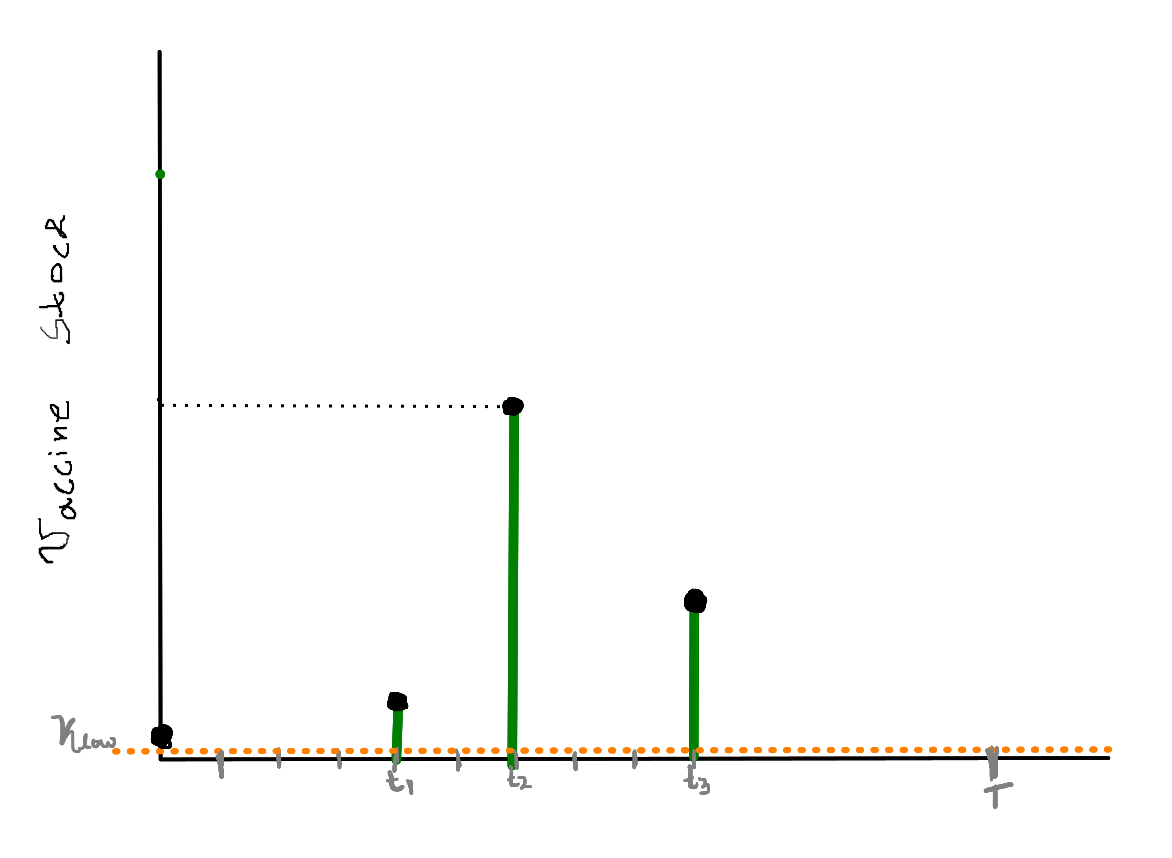
\includegraphics[%
                        width=\textwidth,%
                        keepaspectratio=true]{images/Fig01_000.png}
                }
                \only<2>{
                    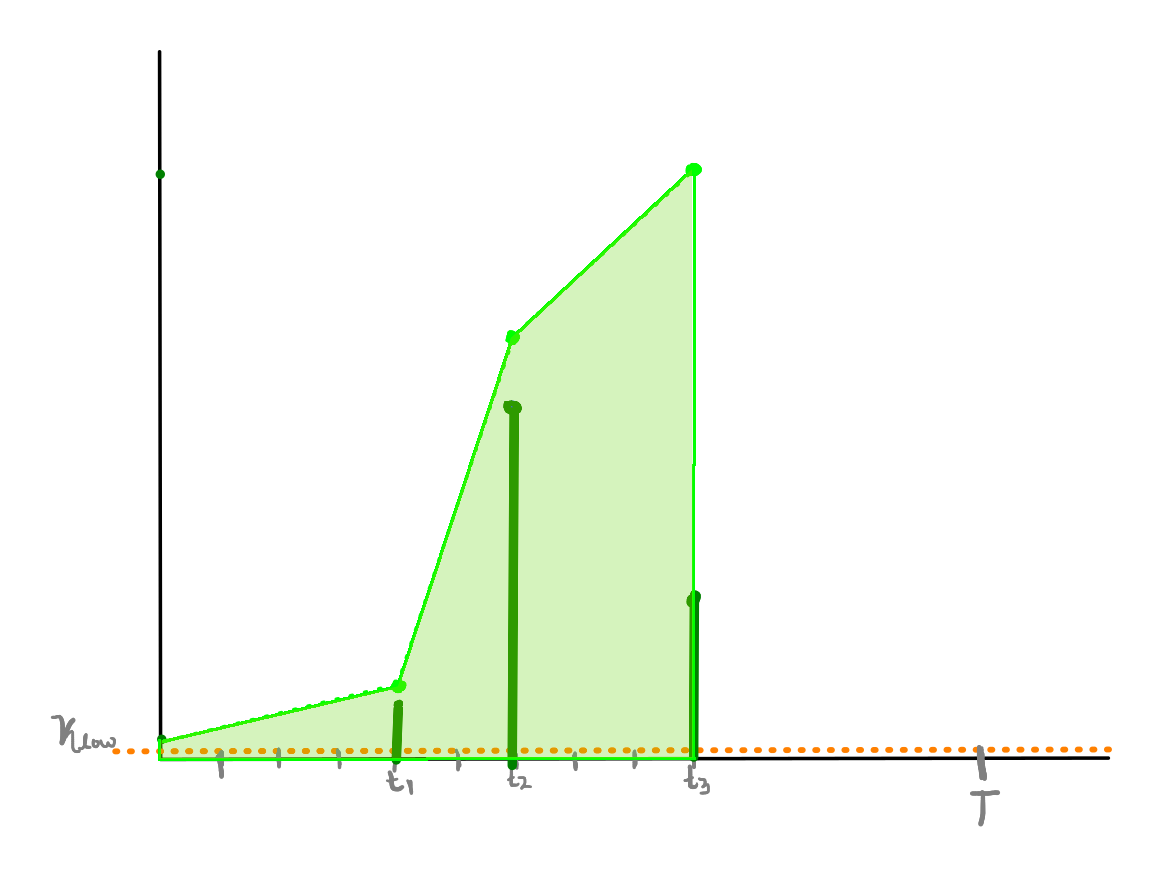
\includegraphics[%
                        width=\textwidth,%
                        keepaspectratio=true]{images/Fig01_001.png}
                }
                \only<3>{
                    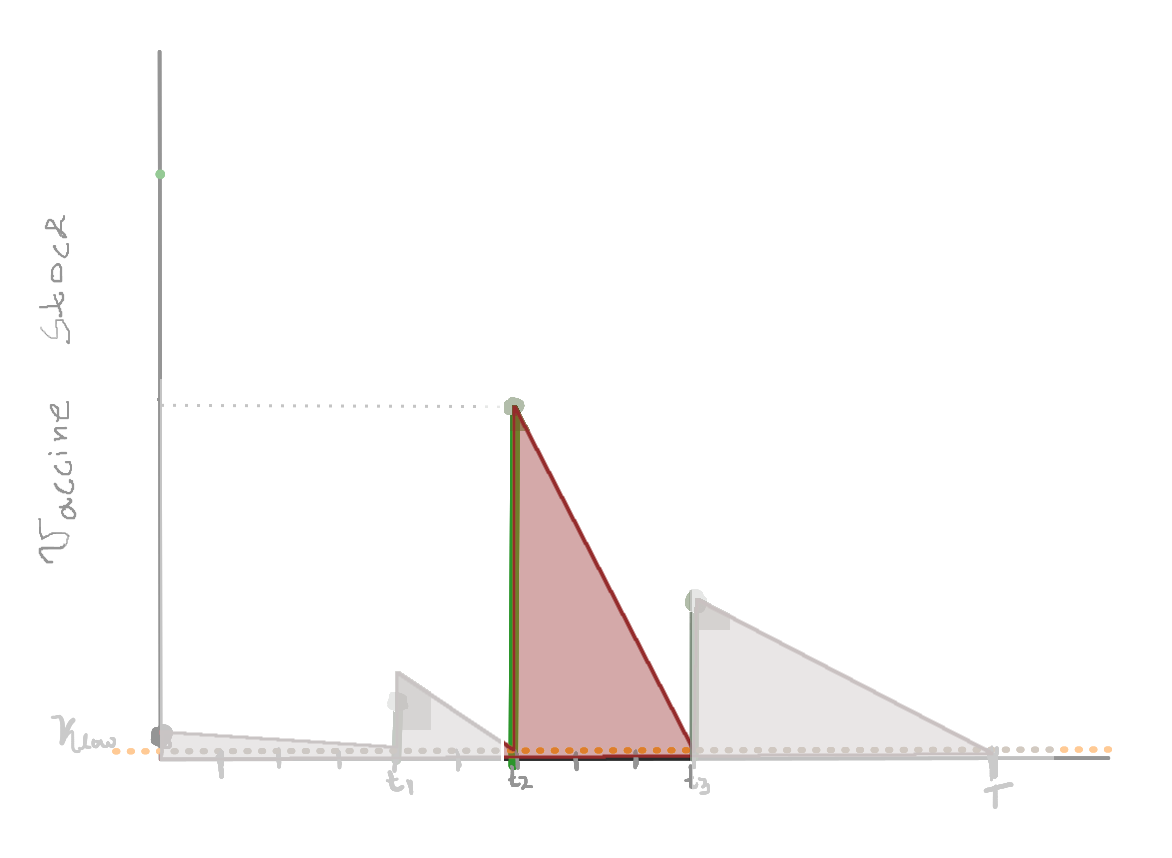
\includegraphics[%
                        width=\textwidth,%
                        keepaspectratio=true]{images/Fig01_002_00.png}
                }

                \only<4-5>{
                    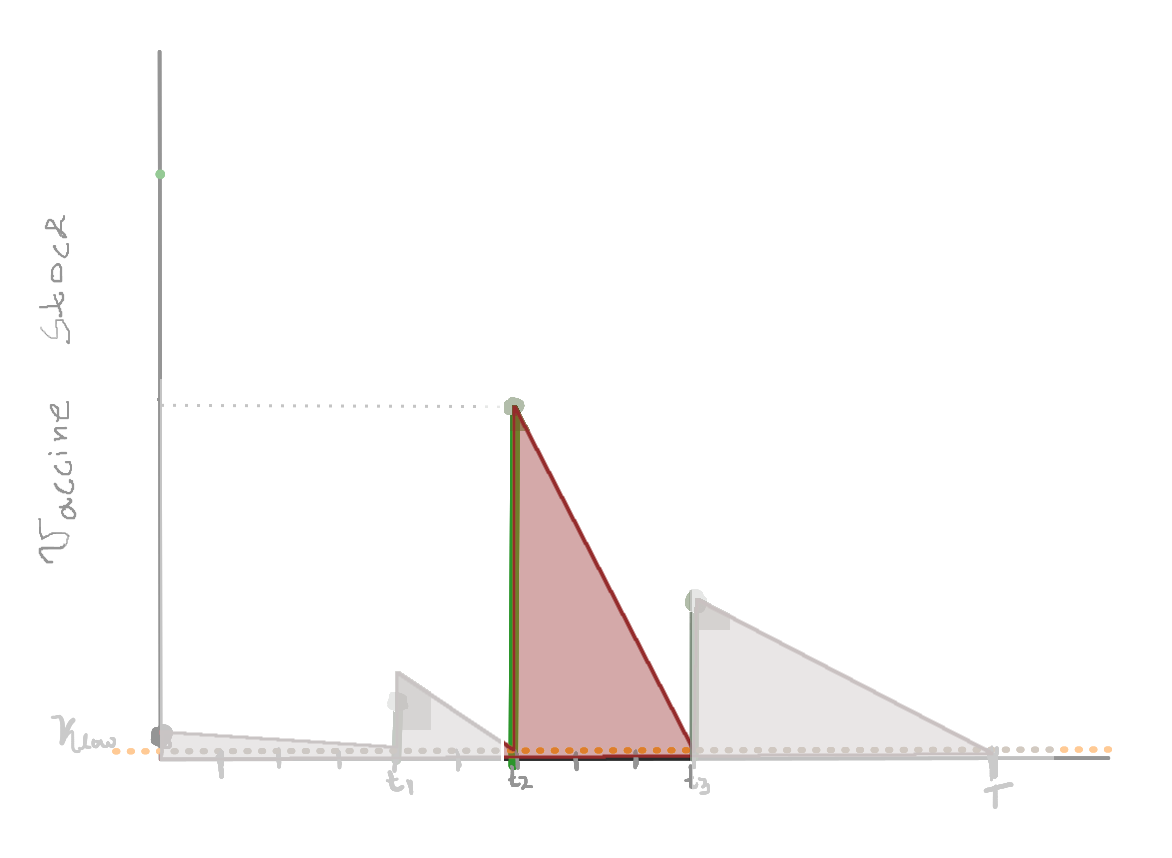
\includegraphics[%
                        width=.7\textwidth,%
                        keepaspectratio=true]{images/Fig01_002_00.png}
                }
%
                \only<6-8>{
                    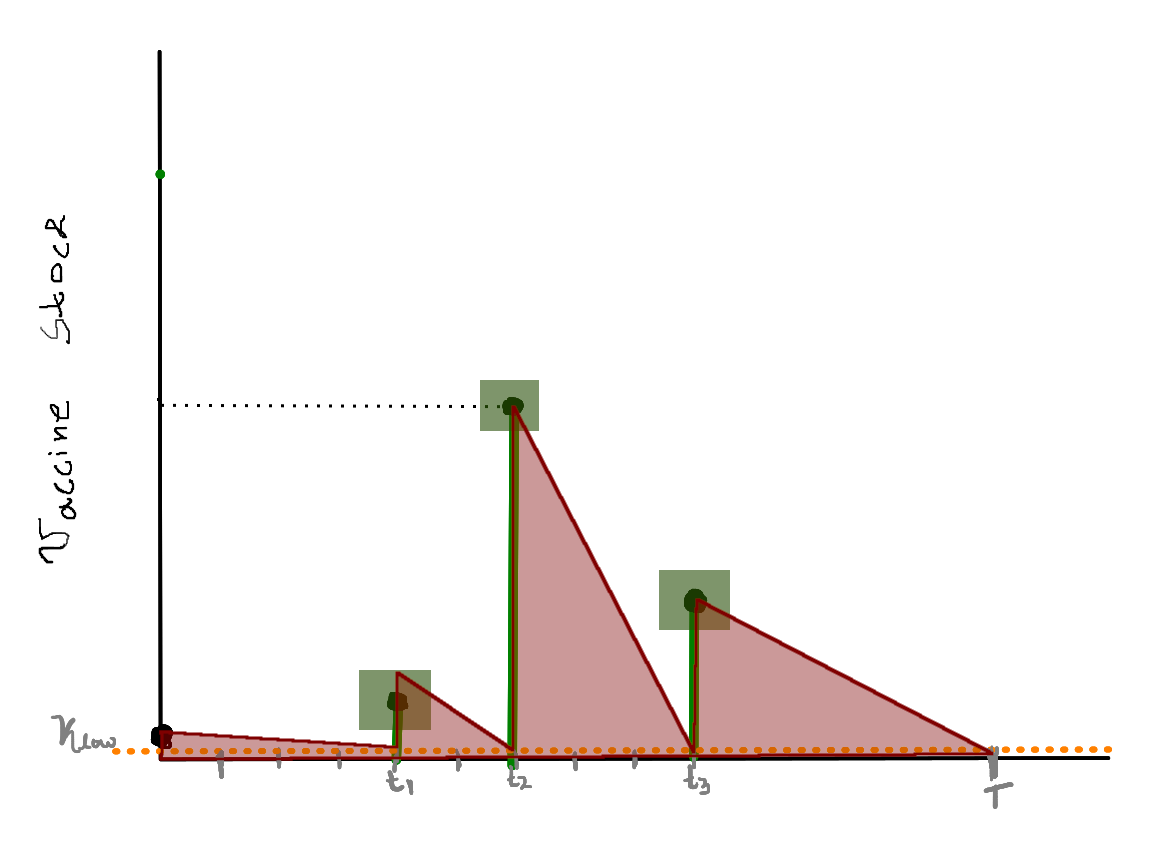
\includegraphics[%
                        width=.7\textwidth,%
                        keepaspectratio=true]{images/Fig01_002.png}
                }
                \only<9>{
                    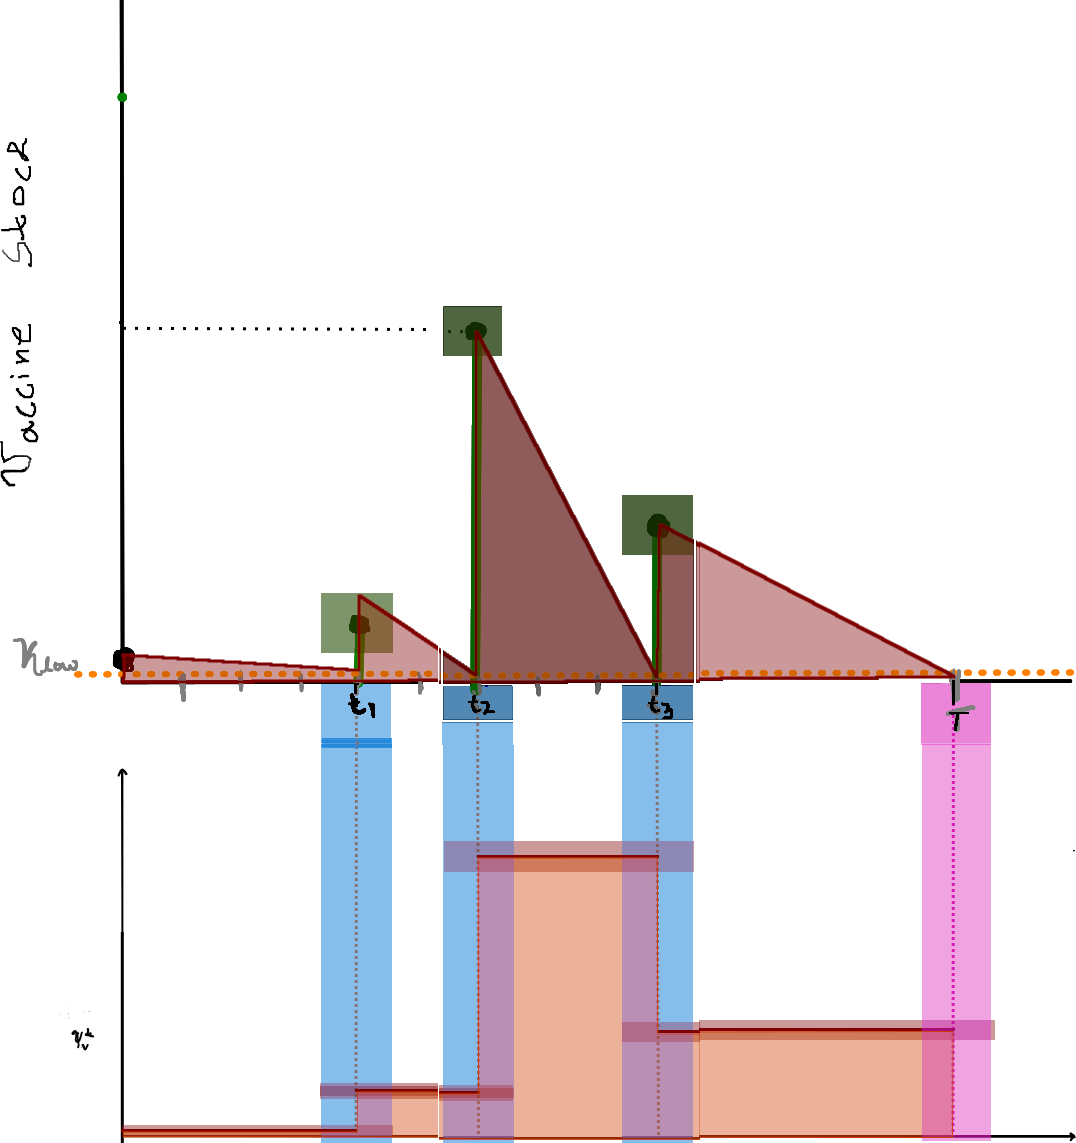
\includegraphics[%
                        width=.65\textwidth,%
                        keepaspectratio=true]{images/Fig01_004_00.png}
                }
                \only<10>{
                    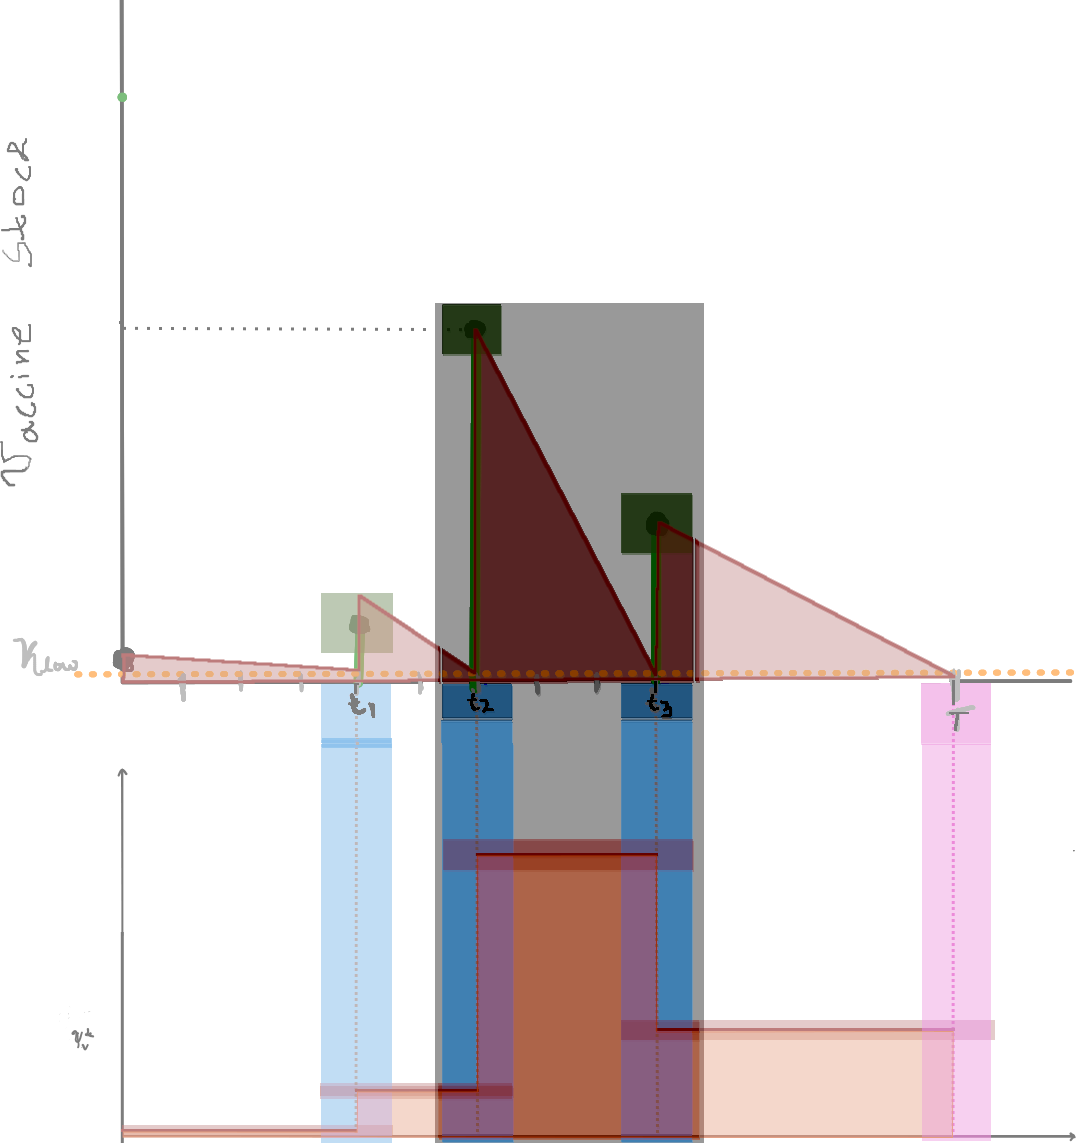
\includegraphics[%
                        width=.65\textwidth,%
                        keepaspectratio=true]{images/Fig01_004_01.png}
                }
                \end{center}
            \end{overlayarea}
        \end{textblock*}
    \begin{textblock*}{120mm}(0mm,57mm)
        \begin{center}
            \only<5-6>{
                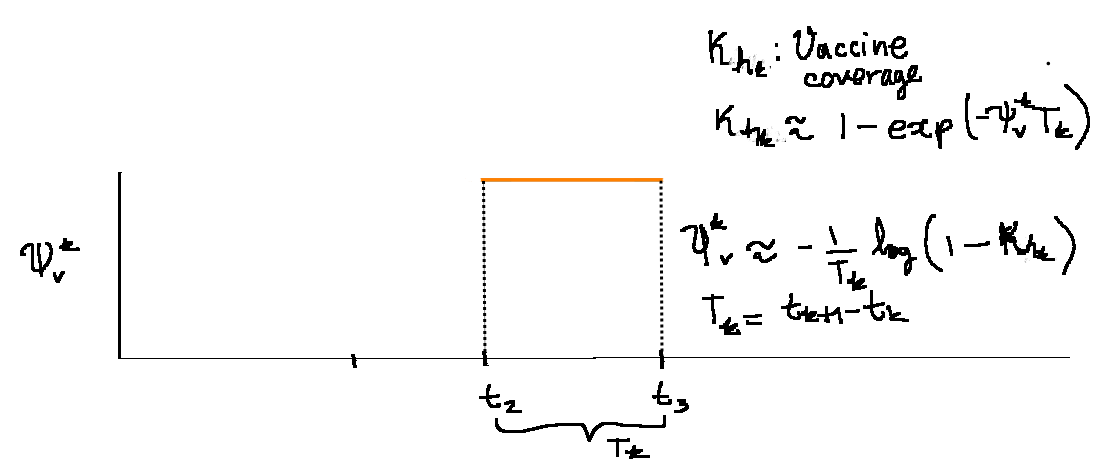
\includegraphics[%
                        width=0.65\textwidth,%
                        keepaspectratio=true]{images/Fig01_002_01.png}
            }
            \only<7>{
                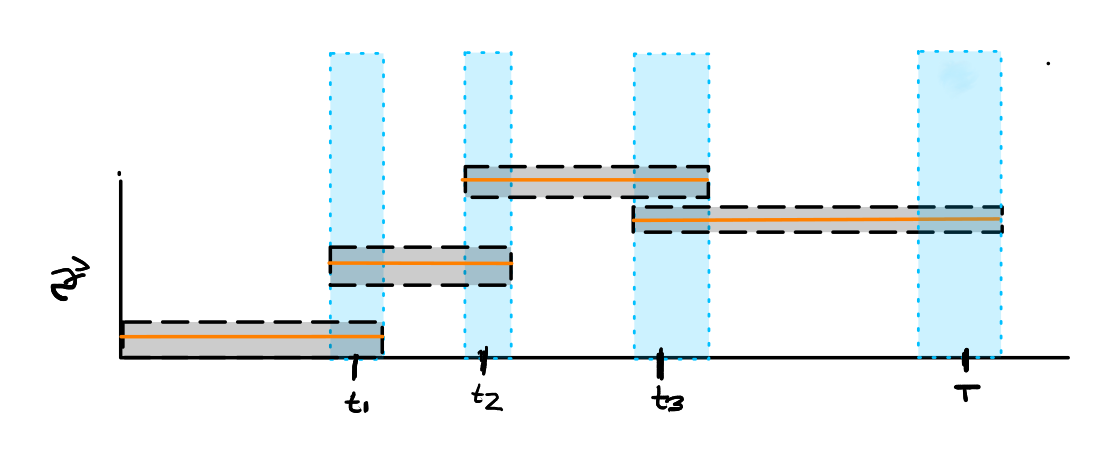
\includegraphics[%
                        width=0.65\textwidth,%
                        keepaspectratio=true]{images/Fig01_002_02.png}
            }
            \only<8>{
                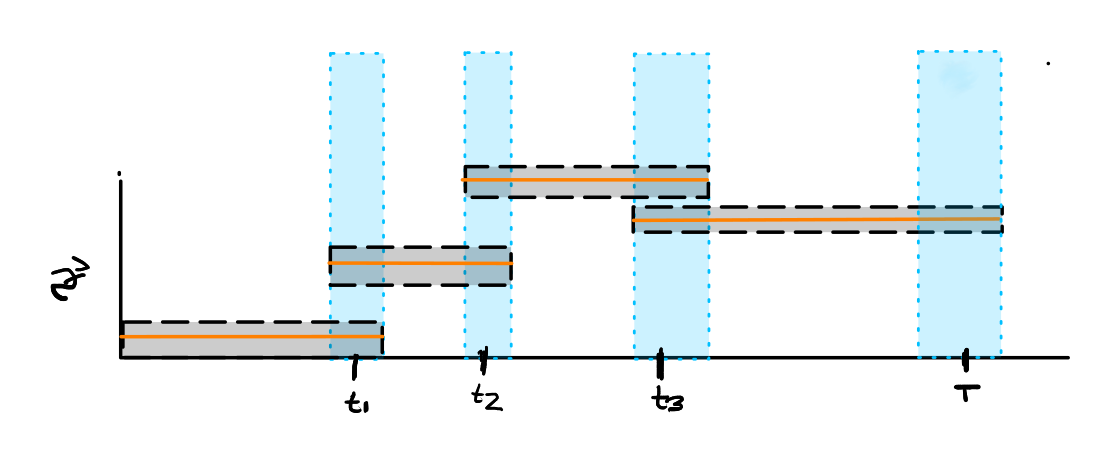
\includegraphics[%
                    width=.65\textwidth,%
                    keepaspectratio=true]{images/Fig01_003.png}
            }
        \end{center}
    \end{textblock*}
\end{frame}
%%%%%%
\begin{frame}{Model Scheme}
    \setlength{\leftmargini}{1mm}
    %!TEX root = ../main.tex
        \setlength{\leftmargini}{1mm}
        \begin{textblock*}{65mm}(5mm, 12mm)
            \only<1>{
                \includegraphics[scale=0.12,%
                    keepaspectratio]{assets/%
                    SchemeModel_withoutVaccination.png}
            }
            \only<2>{
                \includegraphics[scale=0.12,%
                    keepaspectratio]{assets/%
                    SchemeModel_withoutVaccination00.png}
            }
            \only<3->{
                \includegraphics[scale=0.12,%
                    keepaspectratio]{assets/%
                    SchemeModel_withoutVaccination01.png}
            }
        \end{textblock*}
%
    \begin{textblock*}{45mm}(82mm, 50mm)
        \only<2-4>{
            \begin{bluebox}{Vaccine Hypotheses}
                \begin{itemize}
                    %TODO: change bullet indentation
                    \item
                        Imperfect preventive
                    \item
                        One dose
                    \item
                        Symptomatic exception
                    \item
                        Action over susceptible
                \end{itemize}
            \end{bluebox}
        }
    \end{textblock*}
    \begin{textblock*}{75mm}(5mm, 65mm)
    \only<4->{
        \begin{bluebox}{Notation}
            \begin{tabular}{rl}
                $\epsilon$
                & vaccine efficacy
                \\
                $p$
                & Generation of symptoms  probability
                % \\
                % $u_V(t)$
                % & Optimal vaccination policy
            \end{tabular}
        \end{bluebox}
        }
    \end{textblock*}
%
    \begin{textblock*}{45mm}(82mm, 45mm)
        \only<5->{
            \begin{bluebox}{SAGE objectives}
                \begin{itemize}
                    \item
                        Vaccine profile \\(Efficacy, immunity)
                    \item
                        Coverage
                    \item
                        Time Horizon
                \end{itemize}
                \tcblower
                \only<6->{
                    Immunity:
                    \begin{itemize}
                        \item
                            natural (reinfection)
                        \item
                            vaccine-induced
                    \end{itemize}
                }
            \end{bluebox}
        }
    \end{textblock*}
\end{frame}
% %
\begin{frame}
    \begin{textblock*}{80mm}(-5mm, 8mm)
        \begin{align*}
            \frac{d S}{dt}
                &=
                \mu \widehat{N}
                - (\lambda_f + \mu + \psi_V) S
                + \omega_V V + \delta_R R
            \\
            \frac{d E}{dt}
                &=
                \lambda_f S +
                (1- \epsilon) V - (\mu + \delta_E) E
            \\
            \frac{d I_S}{dt}
            &=
                p \delta_E E - (\mu + \alpha_S) I_S
            \\
            \frac{d I_A}{dt}
            &= (1- p)\delta_E E
                - (\mu + \alpha_A)I_A
            \\
            \frac{d R}{dt}
                &= (1 - \theta) \alpha_S I_S
                + \alpha_A I_A
                -(\mu + \delta_R) R
            \\
            \frac{d D}{dt}
            &=  \theta \alpha_S I_S
            \\
            \frac{d V}{dt}
                &= \psi_V S -
                \left[
                    (1 - \epsilon ) \lambda_f + \mu + \omega _V
                \right] V
            \\
            X_{vac}^{\prime} &= \psi_V (S + E + I_A + R)
            \\
            \widehat{N} &= S +E+ I_A + I_S + R, \quad
            \widehat{N} + D = 1
            \\
            \lambda_f &:= \frac{\beta_S I_S + \beta_A I_A}{\widehat{N}}
            %\psi(h) &= 1 - e^{-h} (1- \psi(h) \mu) I_A^n
        \end{align*}
    \end{textblock*}
\end{frame}


     \section{Non standar discrete approximation}
         \begin{frame}{Nonstandard Finite Differences: Dynamic consistency}
    \begin{textblock*}{120mm}(10mm, 18mm)
        We study the evolution of SEIR - mitigation model between
        deliveries.%
    Consider for each time sub-interval $k$  a grid time $N_k$ partition of
    sub-interval $[t_{*}^{(k)},t^{*(k)}]$,
    $$
        h_k:= \frac{t^{*(k)} - t_{*}^{(k)}}{N_k}.
    $$
    If $t_n^{(k)}$ denotes the time of the $n$ step SEIR model for the
    $k$ sub-interval, then
    $$
        t_n^{(k)} =
            n h_k \in [t_{*}^{(k)},t^{*(k)}],
            \qquad k = 1,\dots,
            K.
    $$
    \end{textblock*}
    \only<2>{
        \begin{textblock*}{120mm}(10mm, 60mm)
            \begin{bibunit}[apalike]
                \nocite{Jodar2008}
                \putbib
            \end{bibunit}
        \end{textblock*}
    }
    \only<3>{
    \begin{textblock*}{120mm}(10mm, 60mm)
        Also, we use an adaptive functional discretization
        \begin{align*}
            \varphi(h) &:= h +  \mathcal{O}(h^2)
            \\
            \varphi(h) &= \frac{1-\exp(-h)}{h}
        \end{align*}
    \end{textblock*}
    }
\end{frame}
%----------------------------------------------------------------------
\begin{frame}{}
    \begin{textblock*}{120mm}(0mm,20mm)
            \begin{align*}
                \frac{S^{n+1} - S^n}{\varphi(h)}
                    &= \mu \widehat{N}^n
                    - (\lambda_f + \varphi_V^{(k)}) S^{n+1}
                    - \mu S^n + \omega_V V^n + \delta_R R^n
                    \\
                S^{n+1} &=
                    \varphi(h)[
                        \mu \widehat{N}^n
                        - (\lambda_f +  \varphi_V^{(k)}) S^{n+1}
                        - \mu S^n + \omega_V V^n + \delta_R R^n
                    ] + S^n
                    \\
                S^{n+1} &=
                    \frac{
                        (1-\varphi(h) \mu) S^n
                        + \varphi(h)\mu \widehat{N}^n
                        + \varphi(h)[
                            \omega_V V^n
                            + \delta_R R^n
                        ]}{
                                (1 + \varphi(h))
                                (\lambda_f + \Psi_V^{(k)})
                    }
            \end{align*}
    \end{textblock*}
\end{frame}
%
% %
\begin{frame}{Discrete Model}
    \begin{textblock*}{120mm}(0mm,20mm)
     \begin{align*}
        S^{n+1} &=
            \frac{
                (1-\varphi(h) \mu) S^n
                + \varphi(h)\mu \widehat{N}^n
                + \varphi(h)[
                    \omega_V V^n
                    + \delta_R R^n
                ]}{
                        (1 + \varphi(h))
                        (\lambda_f + \Psi_V^{(k)})
            }
         \\
         E^{n+1}
             &=
             \frac{
                 (1- \mu \varphi(h)) E^n
                 + \varphi(h) \lambda_f
                 [
                     S^{n+1} + (1- \epsilon) V^n
                 ]
             }{
                 (1 + \varphi(h)
                 \delta_E)
             }
         \\
     I_S^{n+1}
     &=
         \frac{
             (1 -\varphi(h) \mu) I_S^n
             + \varphi(h) p \delta_E E^{n+1}
         }{
             1 + \varphi(h) \alpha_S
         }
      \\
      &\vdots
      \\
      V^{n+1} &= V^n(1-\varphi(h)[(1 - \epsilon )\lambda_f + \mu + \omega _V]) +
           \varphi(h)(\psi_V^{(k)}) S^{n+1}
      \\
      \\
      X_{vac}^{n+1} &=
               \varphi(h) \psi_V^{\color{orange}{(k)}}
               (S^n + E^n + I_A^n + R^n)
               + X_{vac}^n
      \\
            K^{n+1} &=
                \max \{0, K^n - (X_{vac}^{n+1} - X_k^0 -L)\}
     \end{align*}
    \end{textblock*}
\end{frame}

\begin{frame}{The disability-adjusted life year (DALY)}
    \begin{textblock*}{120mm}(5mm,0mm)
        %
        \begin{graybox}{{$DALY(c,s,a,t) = YLL(c,s,a,t) + YLD(c,s,a,t)$}}
        \only<1-3>{
            For given cause c, age a, sex s and year t
            \begin{description}
                \item[$YLL:$] Years of life lost due to premature death.
                    $$
                        YLL(c,s,a,t) = N(c,s,a,t) \times L(s,a)
                    $$
                    \begin{itemize}
                         \item
                             $N(c,s,a,t):$ is the number of
                             deaths due to the cause $c$
                         \item
                             $L(s,a):$ is a standard loss
                             function specifying years of life lost
                    \end{itemize}
                 \item[$YLD:$] Years of life list due to disability
                     $$
                         YLD(c,s,a,t) = I(c,s,a,t) \times DW(c,s,a)
                         \times L(c,s,a,t)
                     $$
                    \begin{itemize}
                        \item
                            $I(c,s,a,t):$ number of incident cases for cause c
                        \item
                            $DW(c,s,a):$ disability weight for cause c
                        \item
                            $L(c,s,a,t):$  average duration of the case
                    \end{itemize}
            \end{description}
       }
       \end{graybox}
    \end{textblock*}
    \end{frame}
\begin{frame}{}
           \begin{equation*}
                \begin{aligned}
                 & \only<1->{
                    \min_{a_V  \in \mathcal{U}[0, T]}
                 }
                     J(a_V) :=
                 \only<2->{
                    \underbrace{a_D ( D(T) - D(0))}_{:=YLL}  +
                    \underbrace{a_S (Y_{I_S}(T) - Y_{I_S}(0))}_{:=YLD}
                 }
                 \only<3>{
                     \\
                     a_V &:= \{a_{t_0}, a_{t_1}, \cdots, a_{t_K}\}
                     \\
                     a_{t_k} &:= p_k \Psi^k_V,
                     \\
                     s.t. & \quad \{\text{Stock constrains}\}
                 }
                \end{aligned}
           \end{equation*}
\end{frame}
     \section{Numeric Results}
        \begin{frame}{Results: deterministic controlled dynamics}
    \centering
    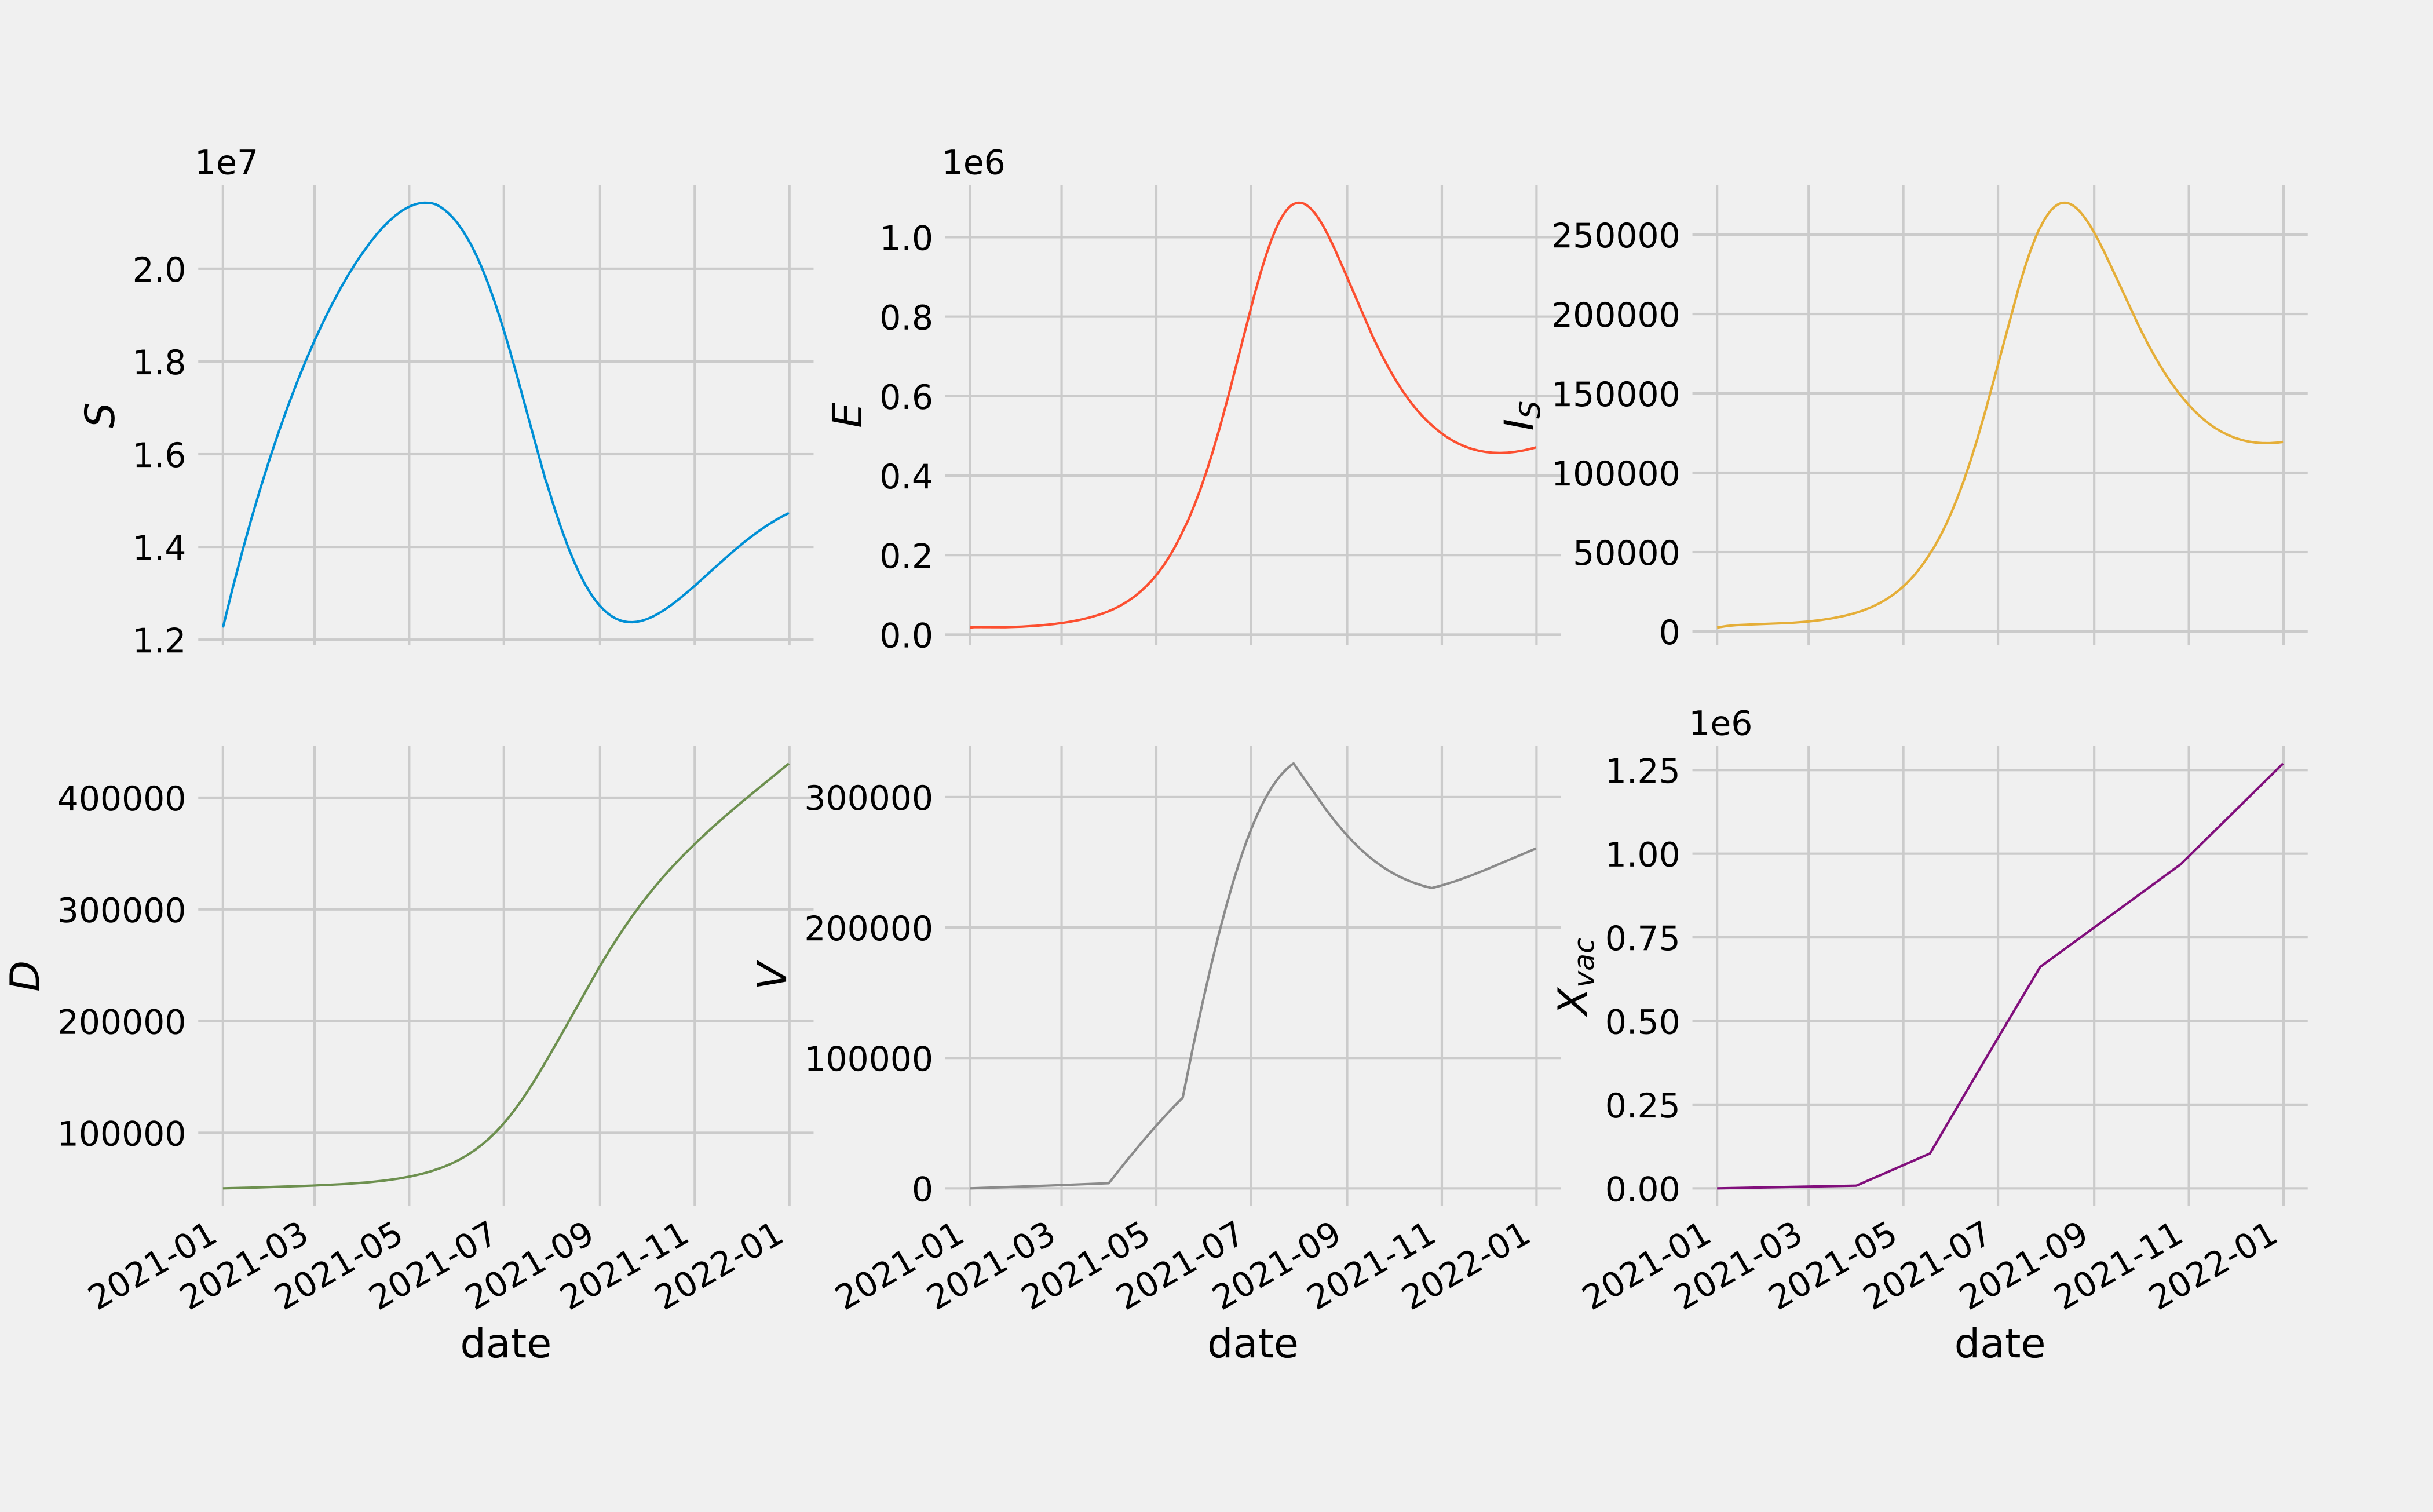
\includegraphics[width=1.05\linewidth]{assets/det_states.png}
\end{frame}

\begin{frame}{Results}
    \centering
    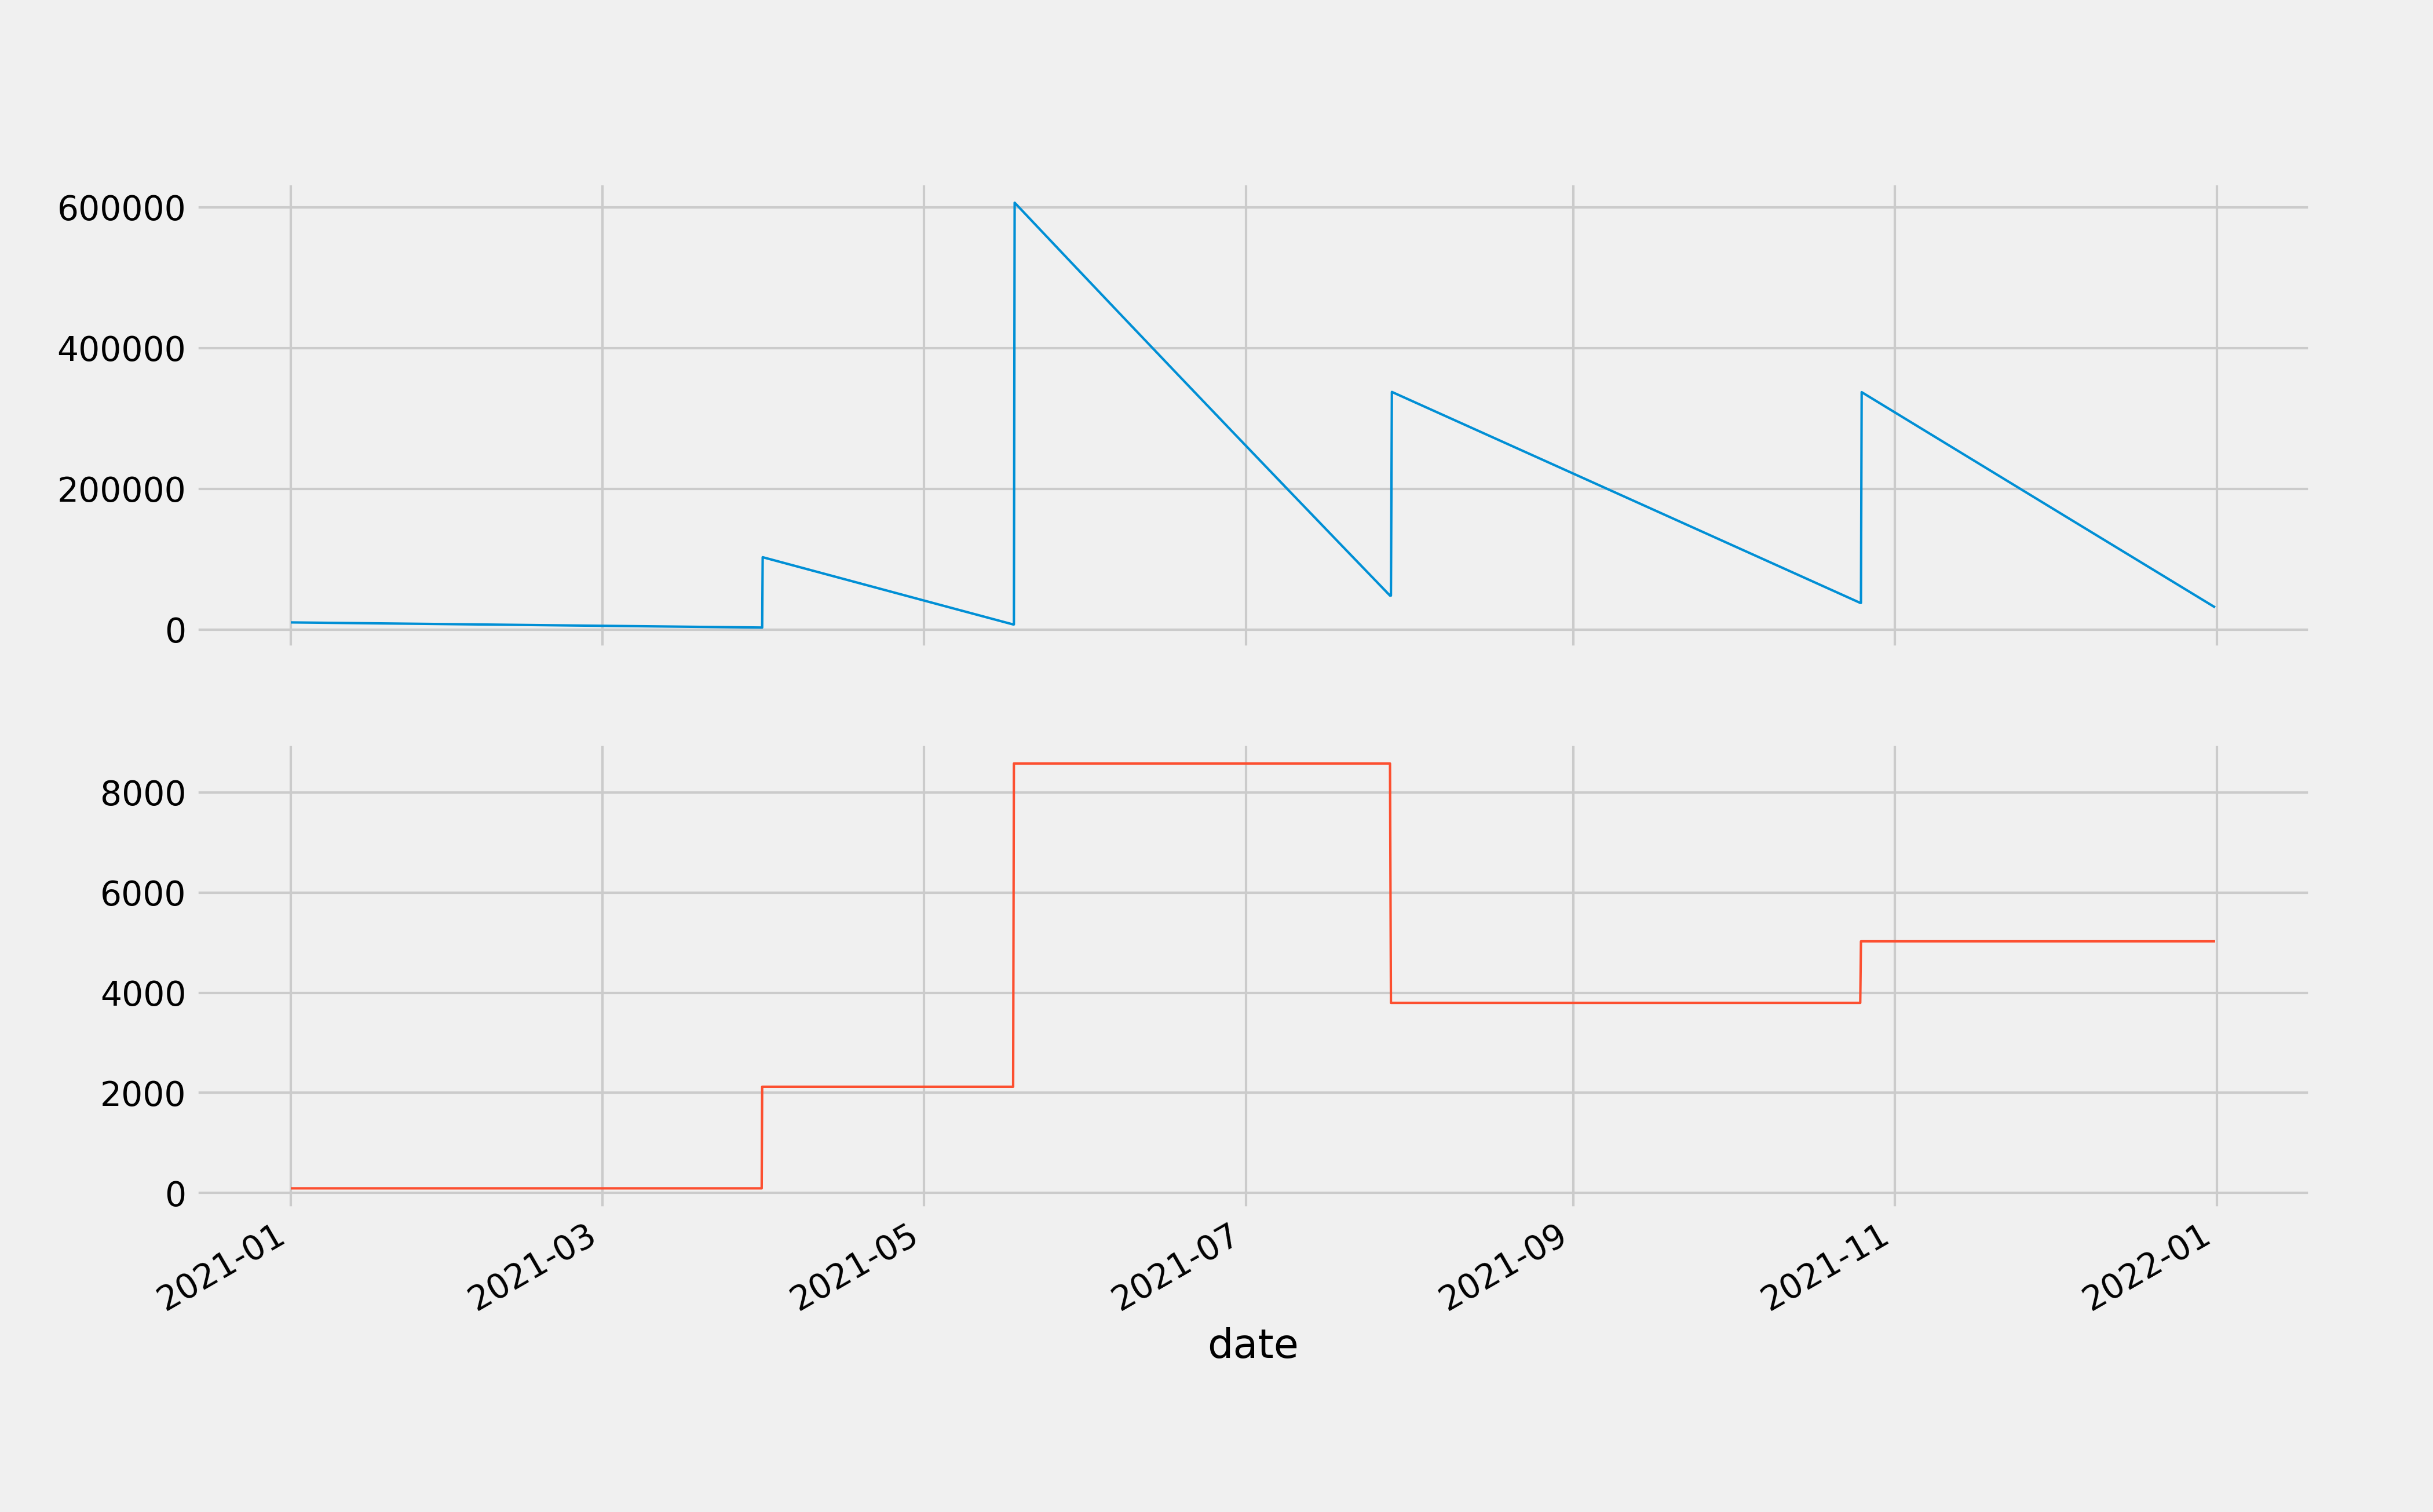
\includegraphics[width=1.05\linewidth]{assets/det_policy.png}
\end{frame}

\begin{frame}{Results: stochatic dynamics}
    \centering
    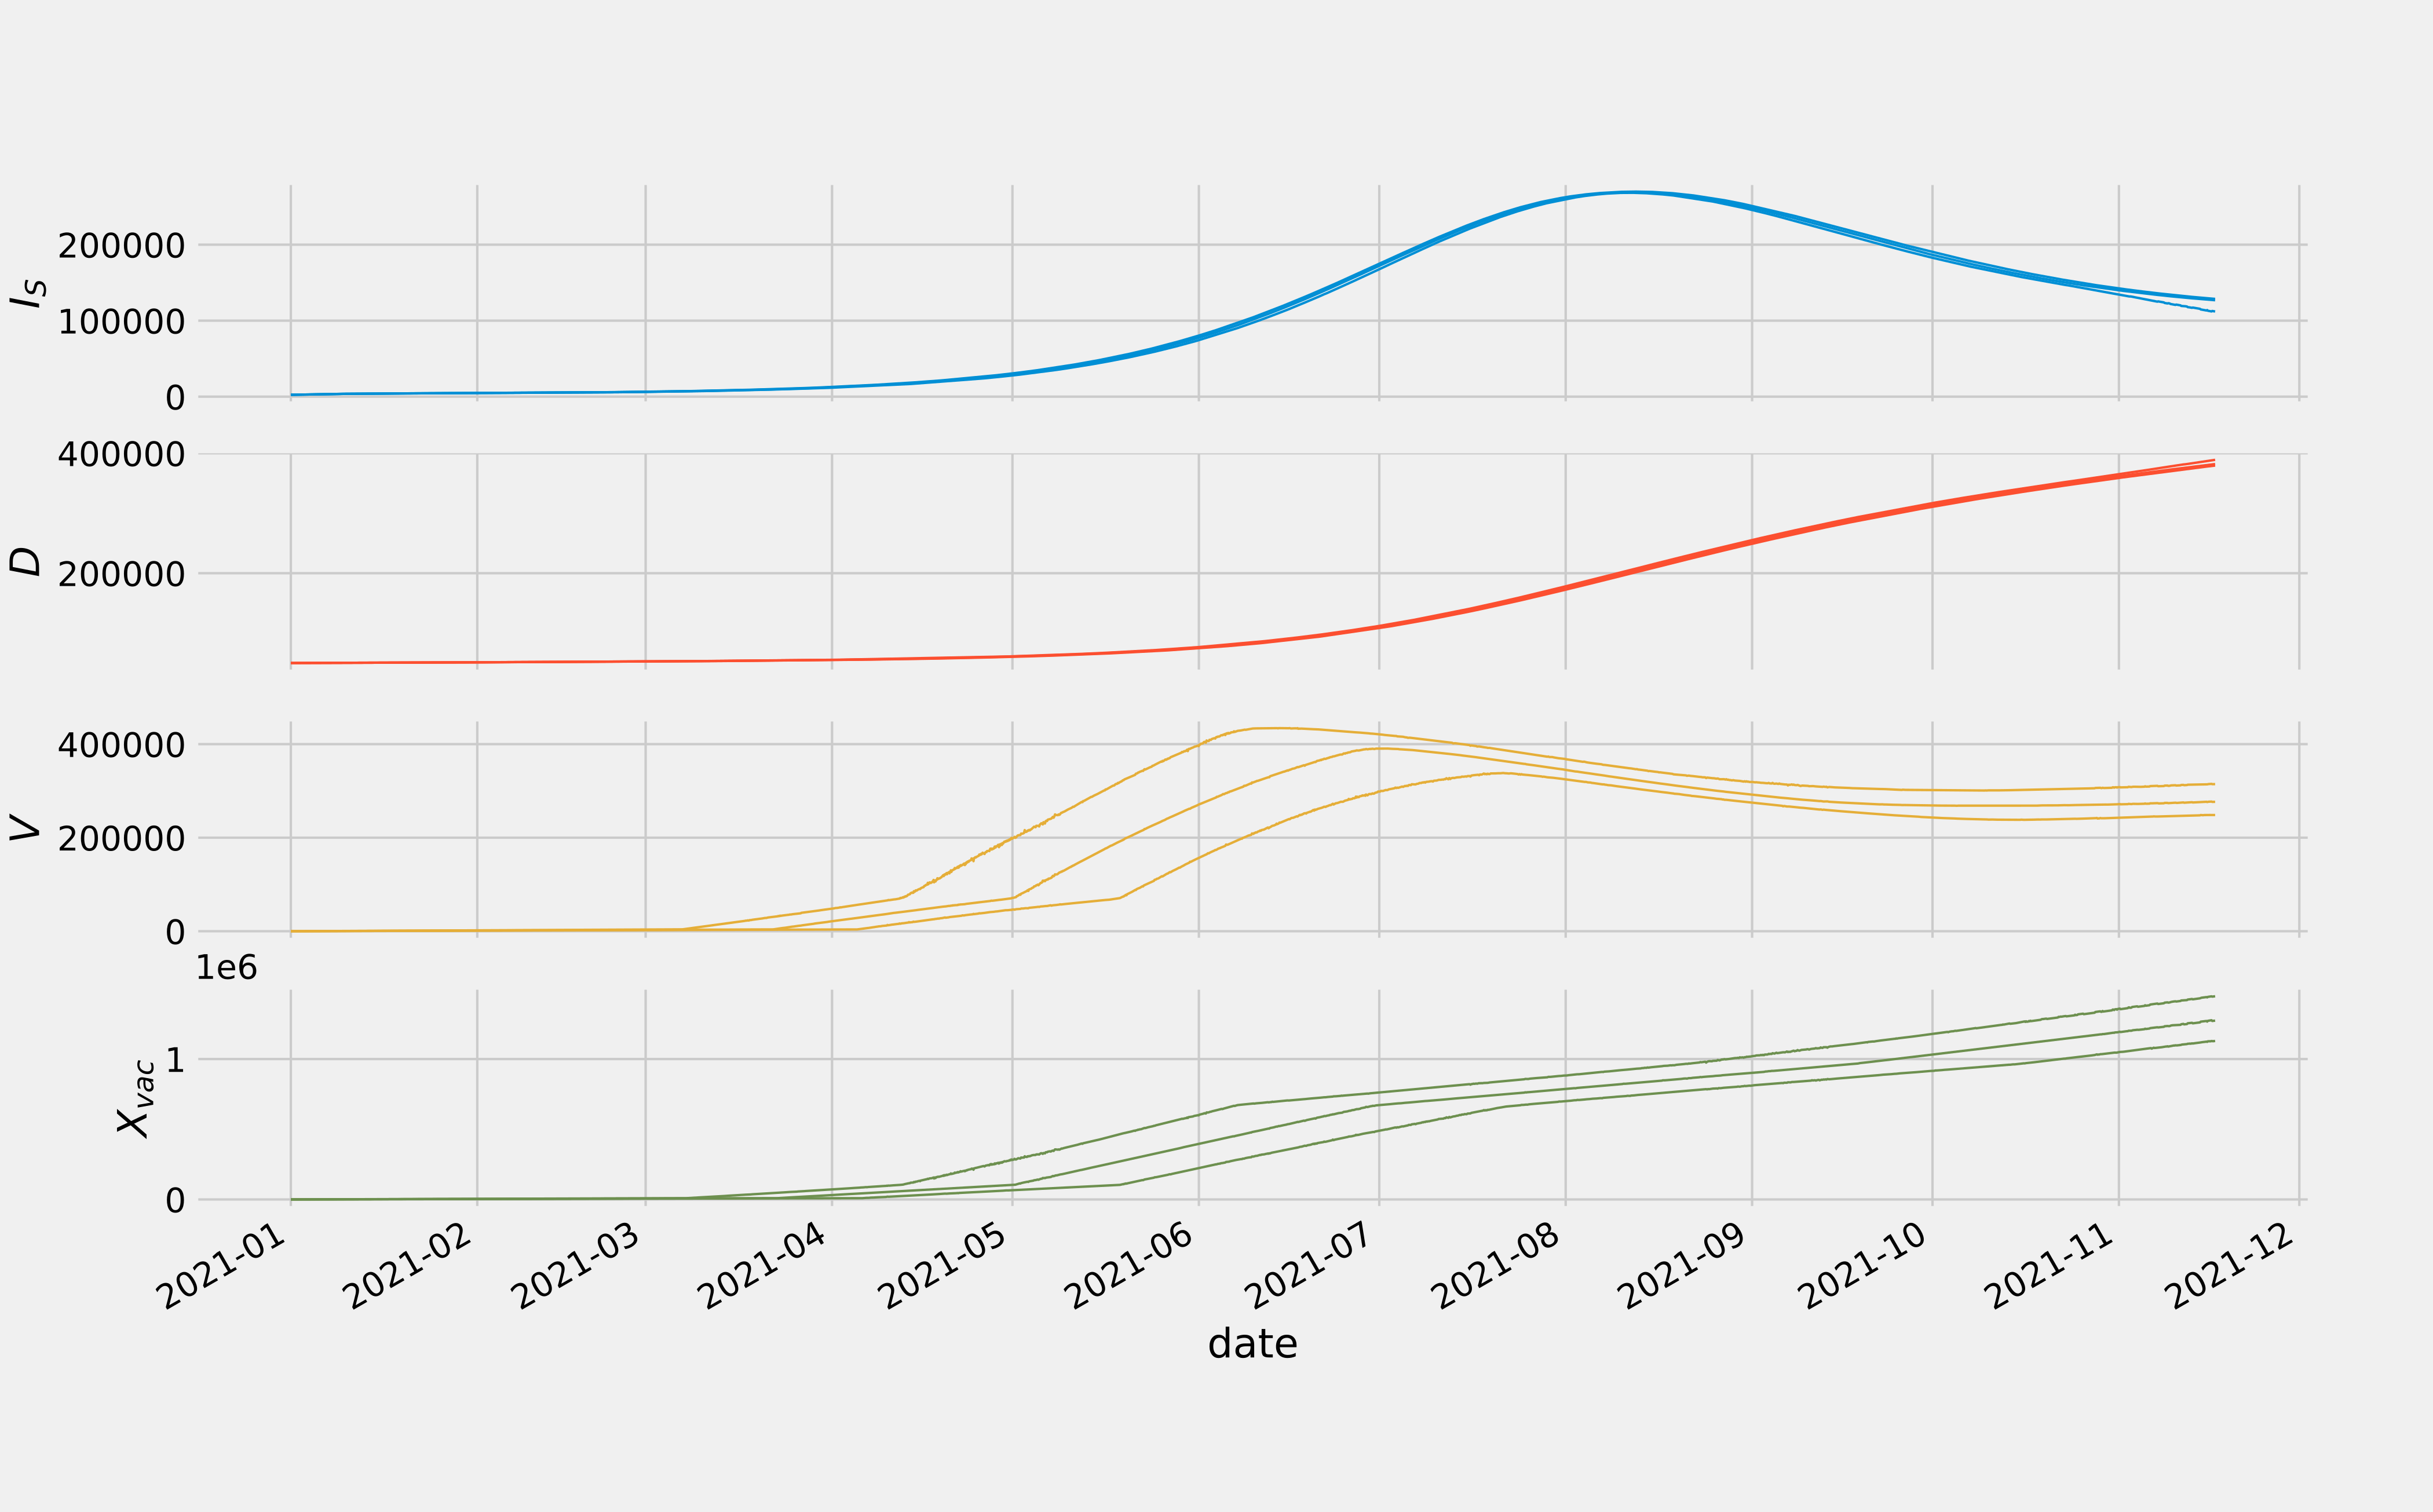
\includegraphics[width=1.05\linewidth]{assets/ci_states.png}
\end{frame}

\begin{frame}{Results: stochatic dynamics}
    \centering
    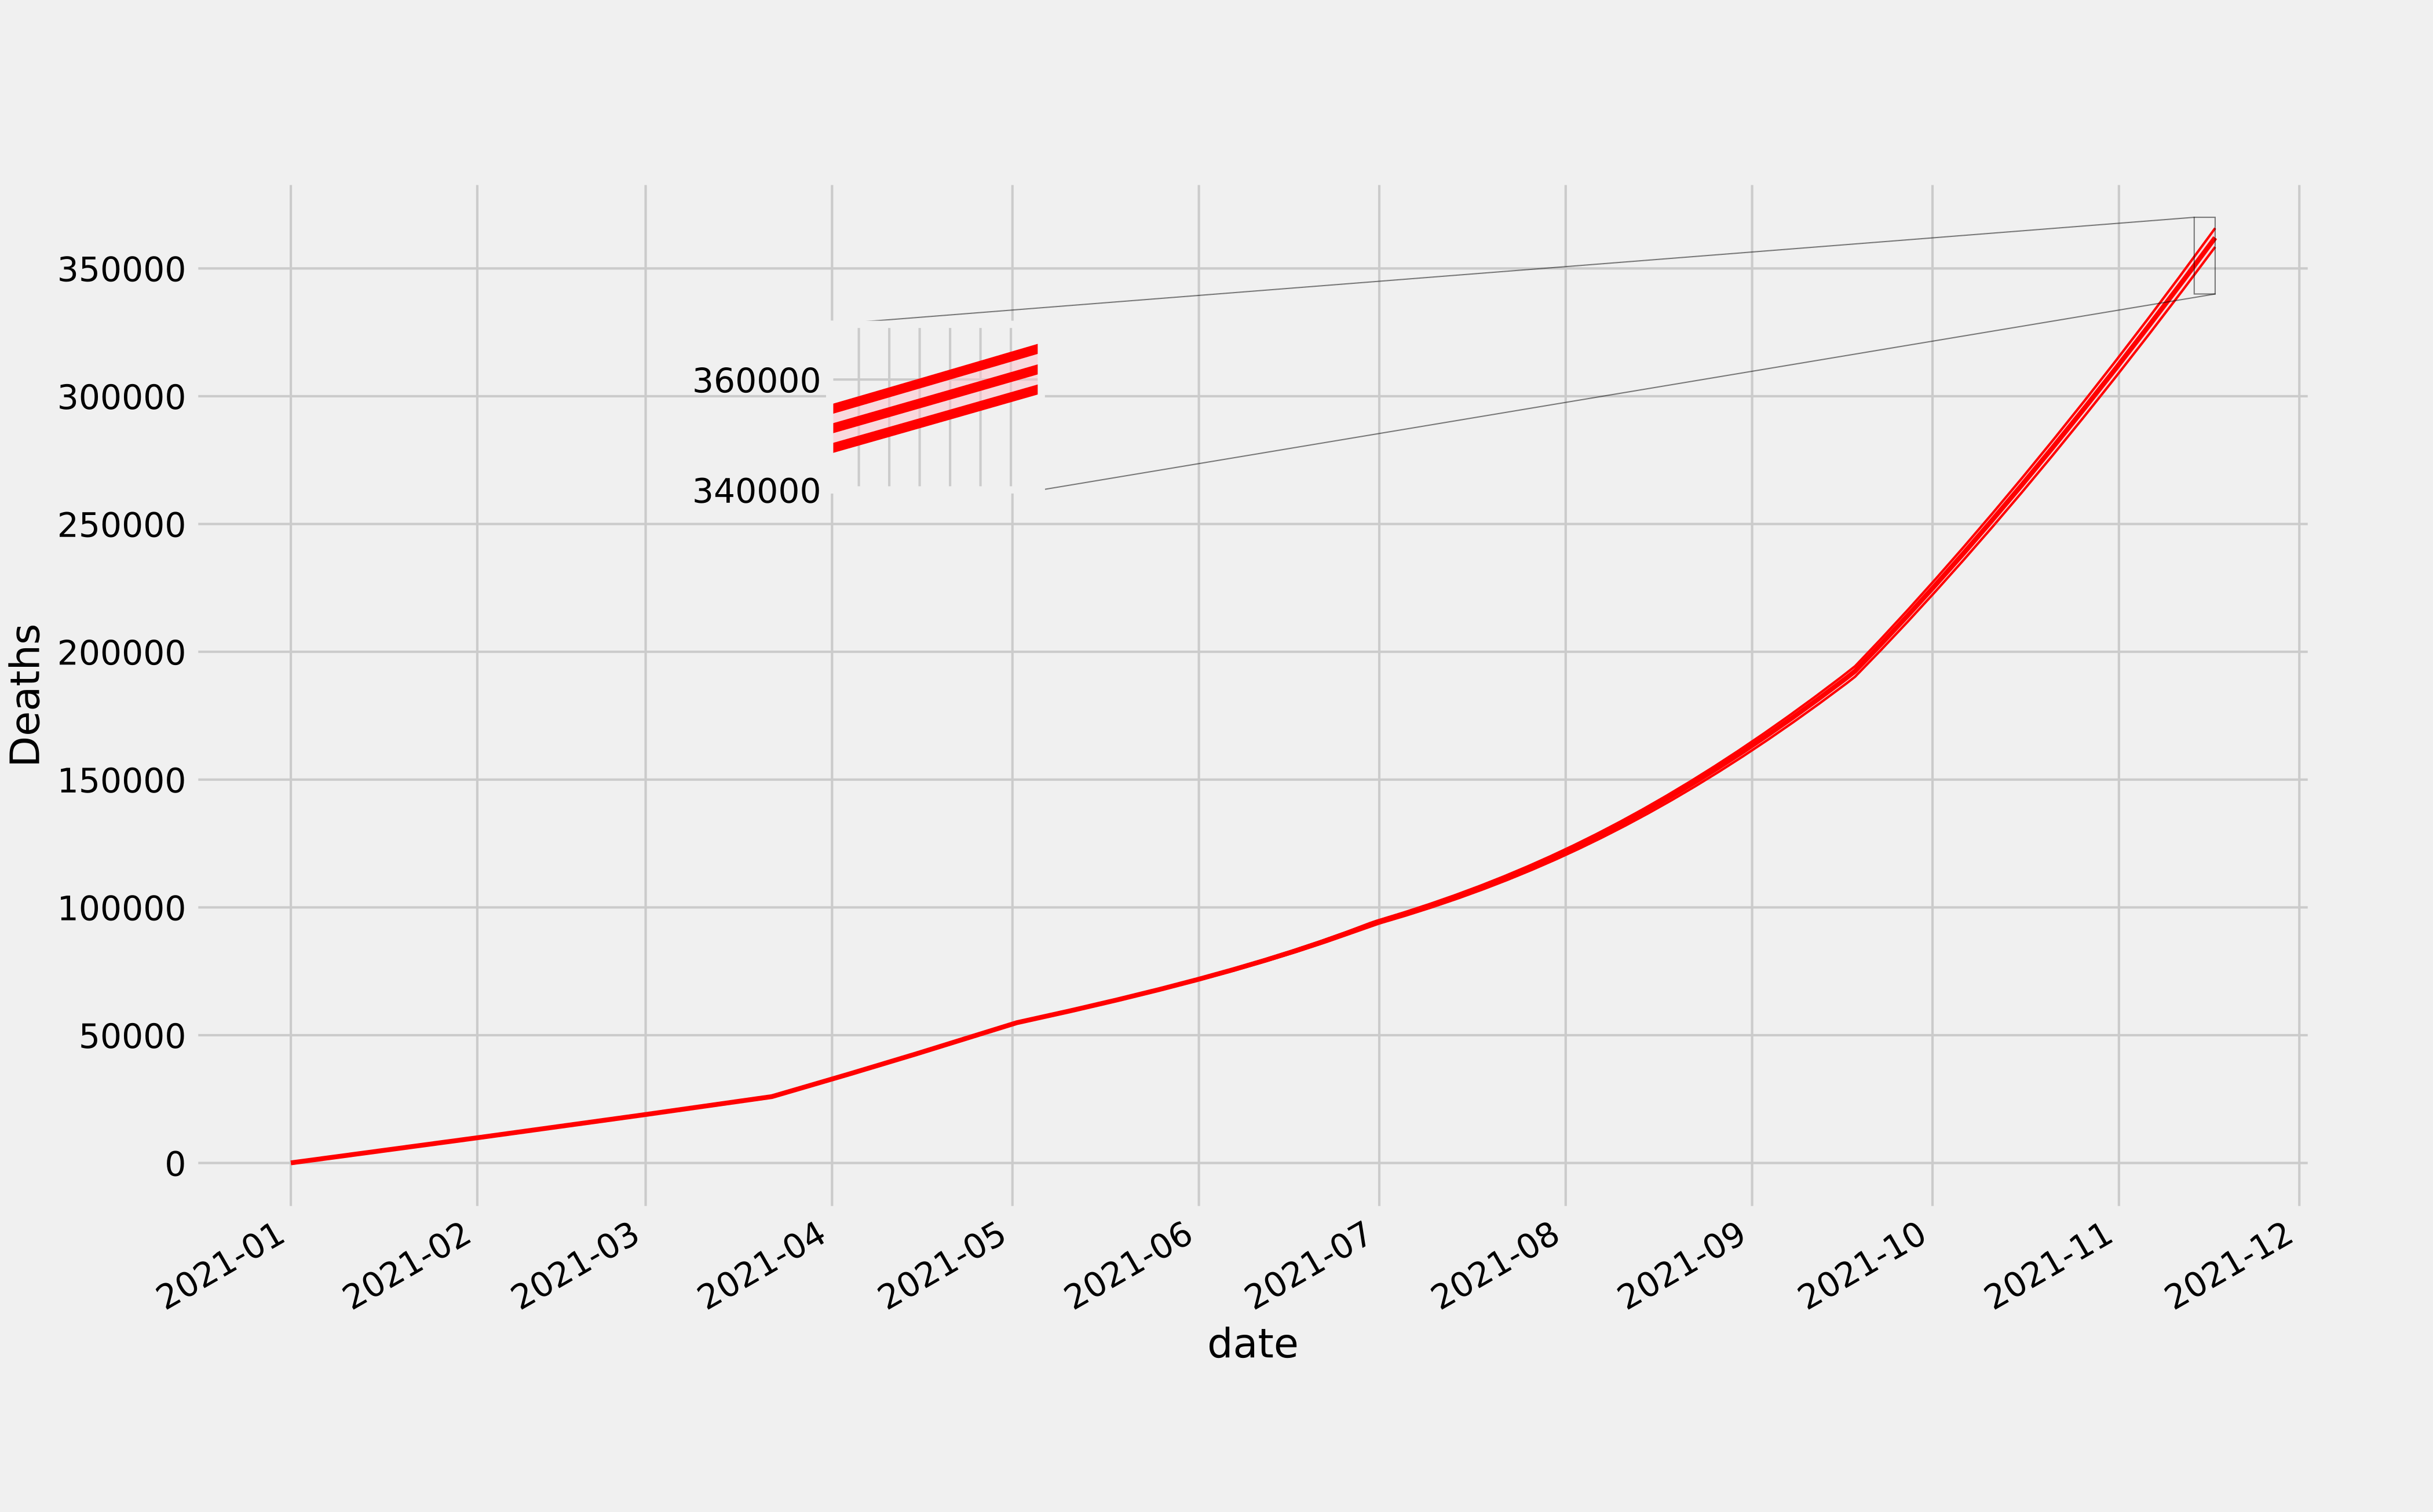
\includegraphics[width=1.05\linewidth]{assets/cumulative_deaths.png}
\end{frame}

\begin{frame}{Results: Stcok CI}
    \centering
    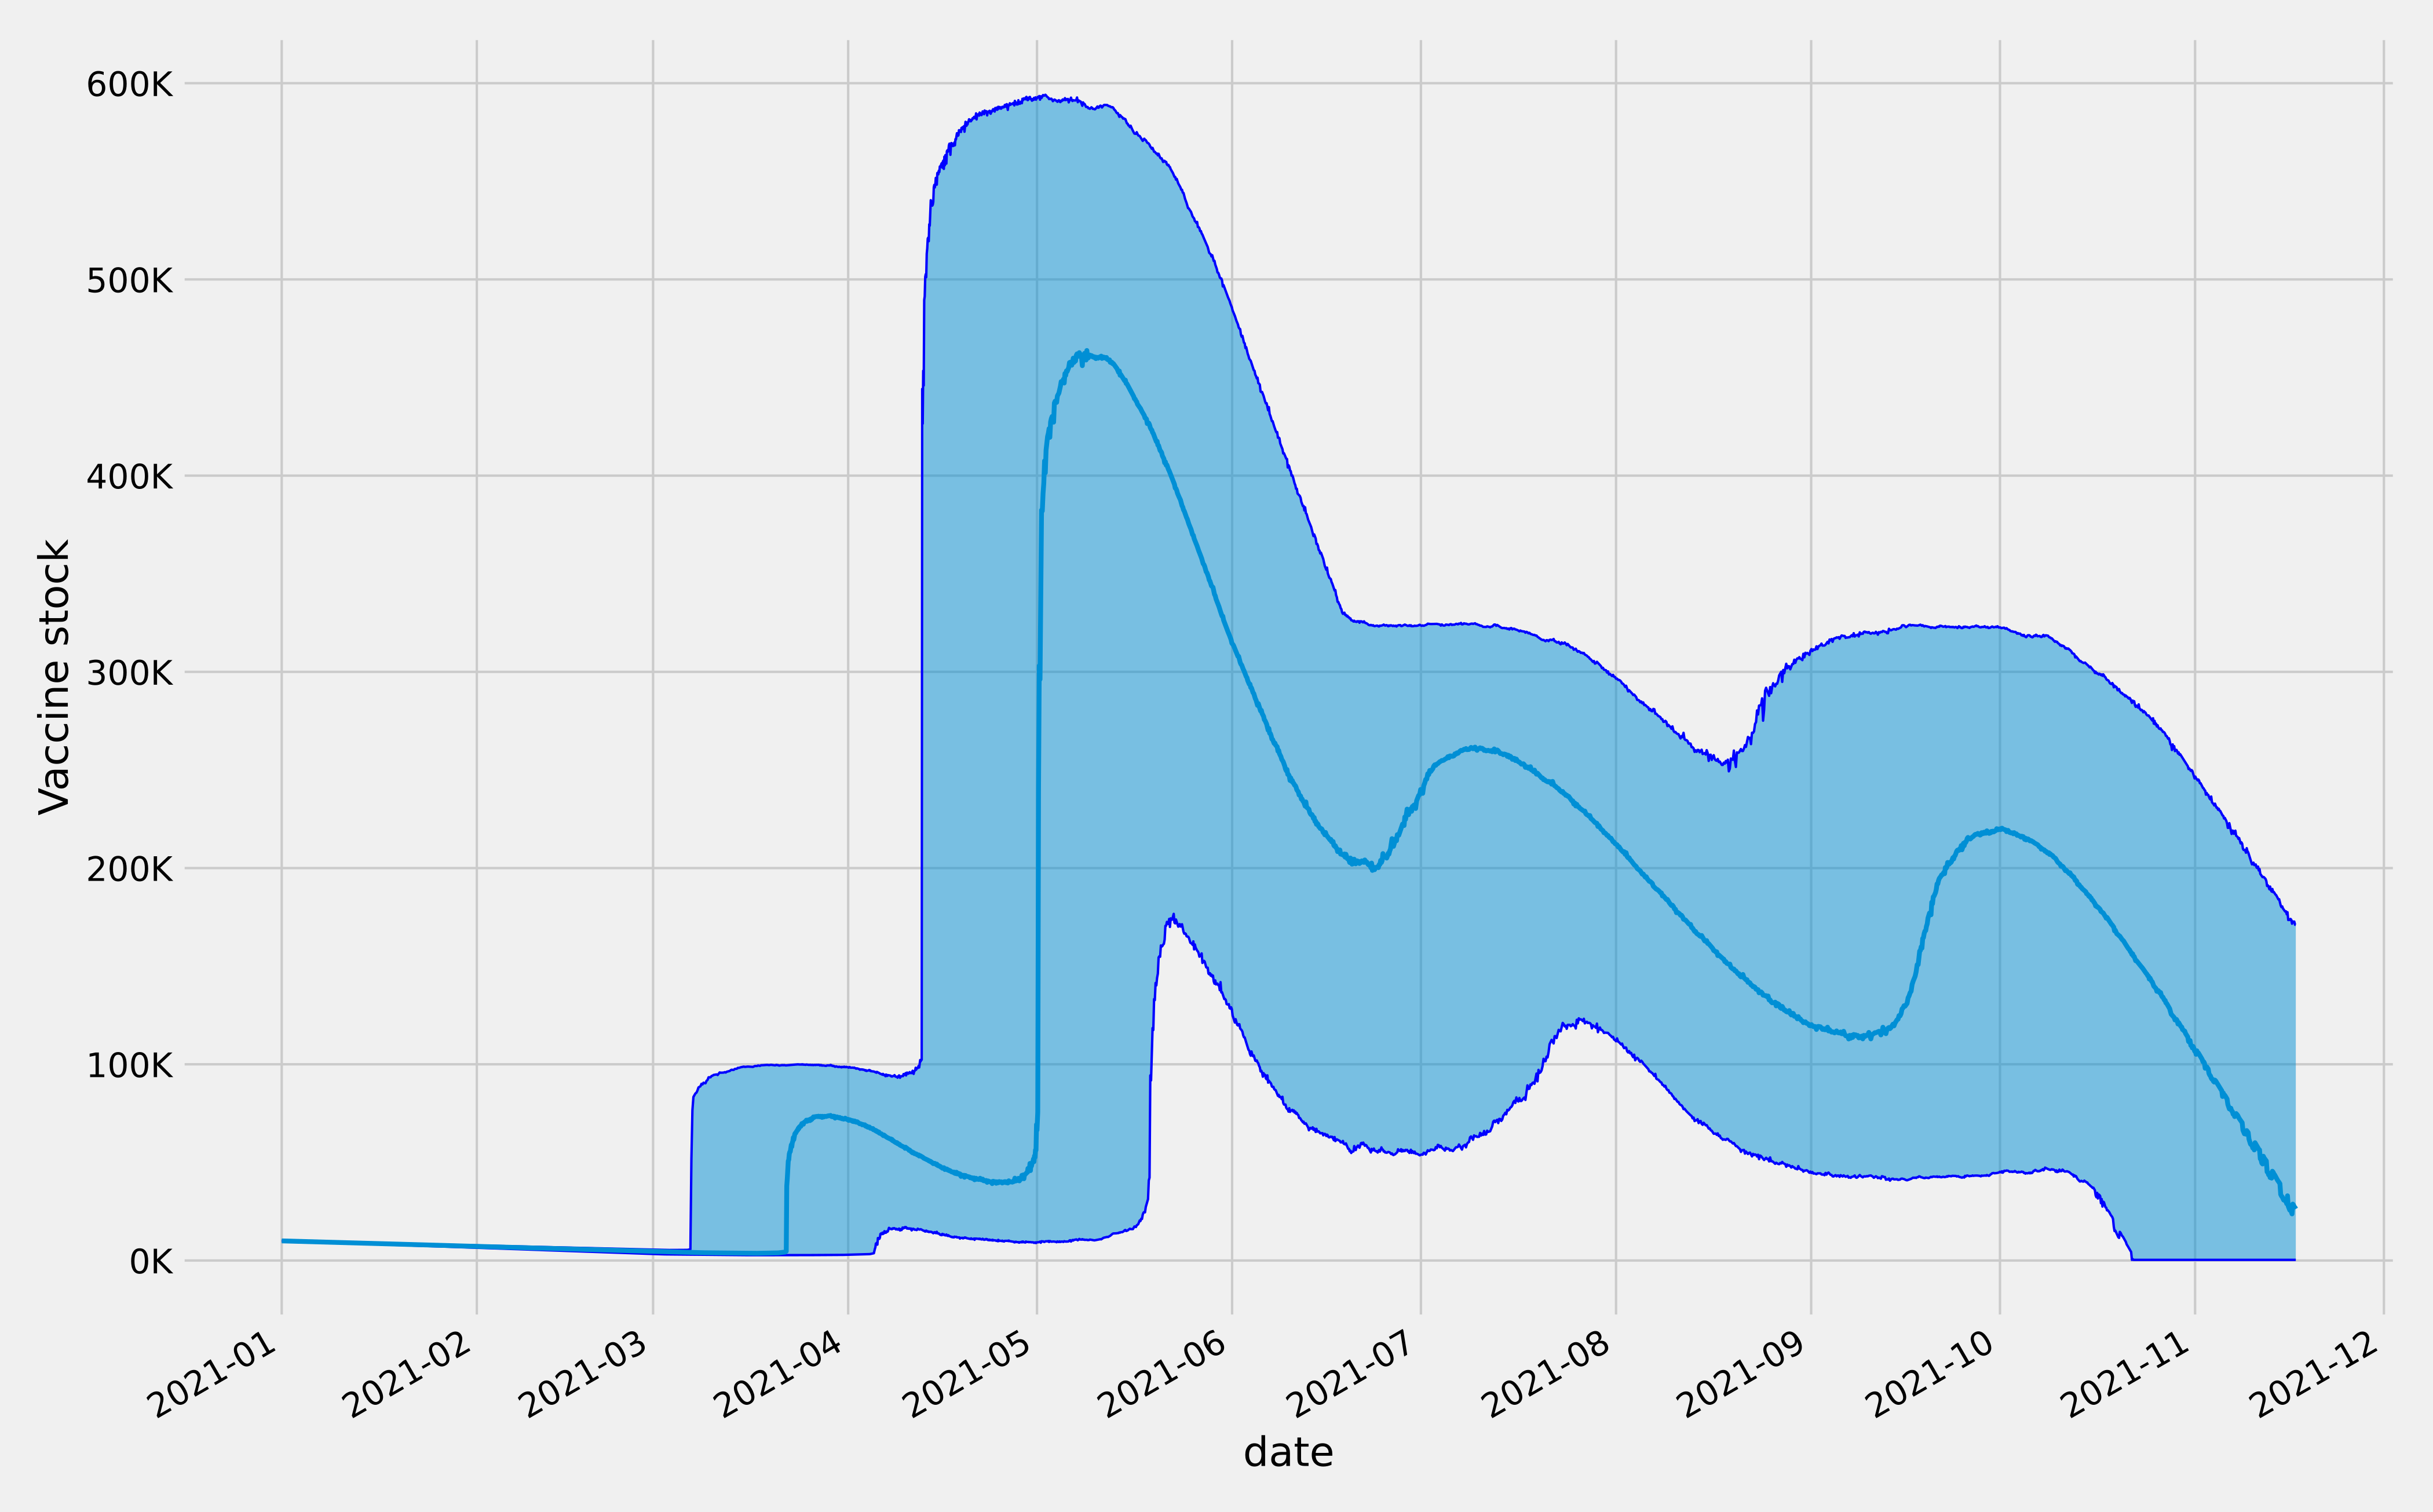
\includegraphics[width=1.05\linewidth]{assets/stock.png}
\end{frame}

\begin{frame}{Results: Actions (vaccination rate) CI}
    \centering
    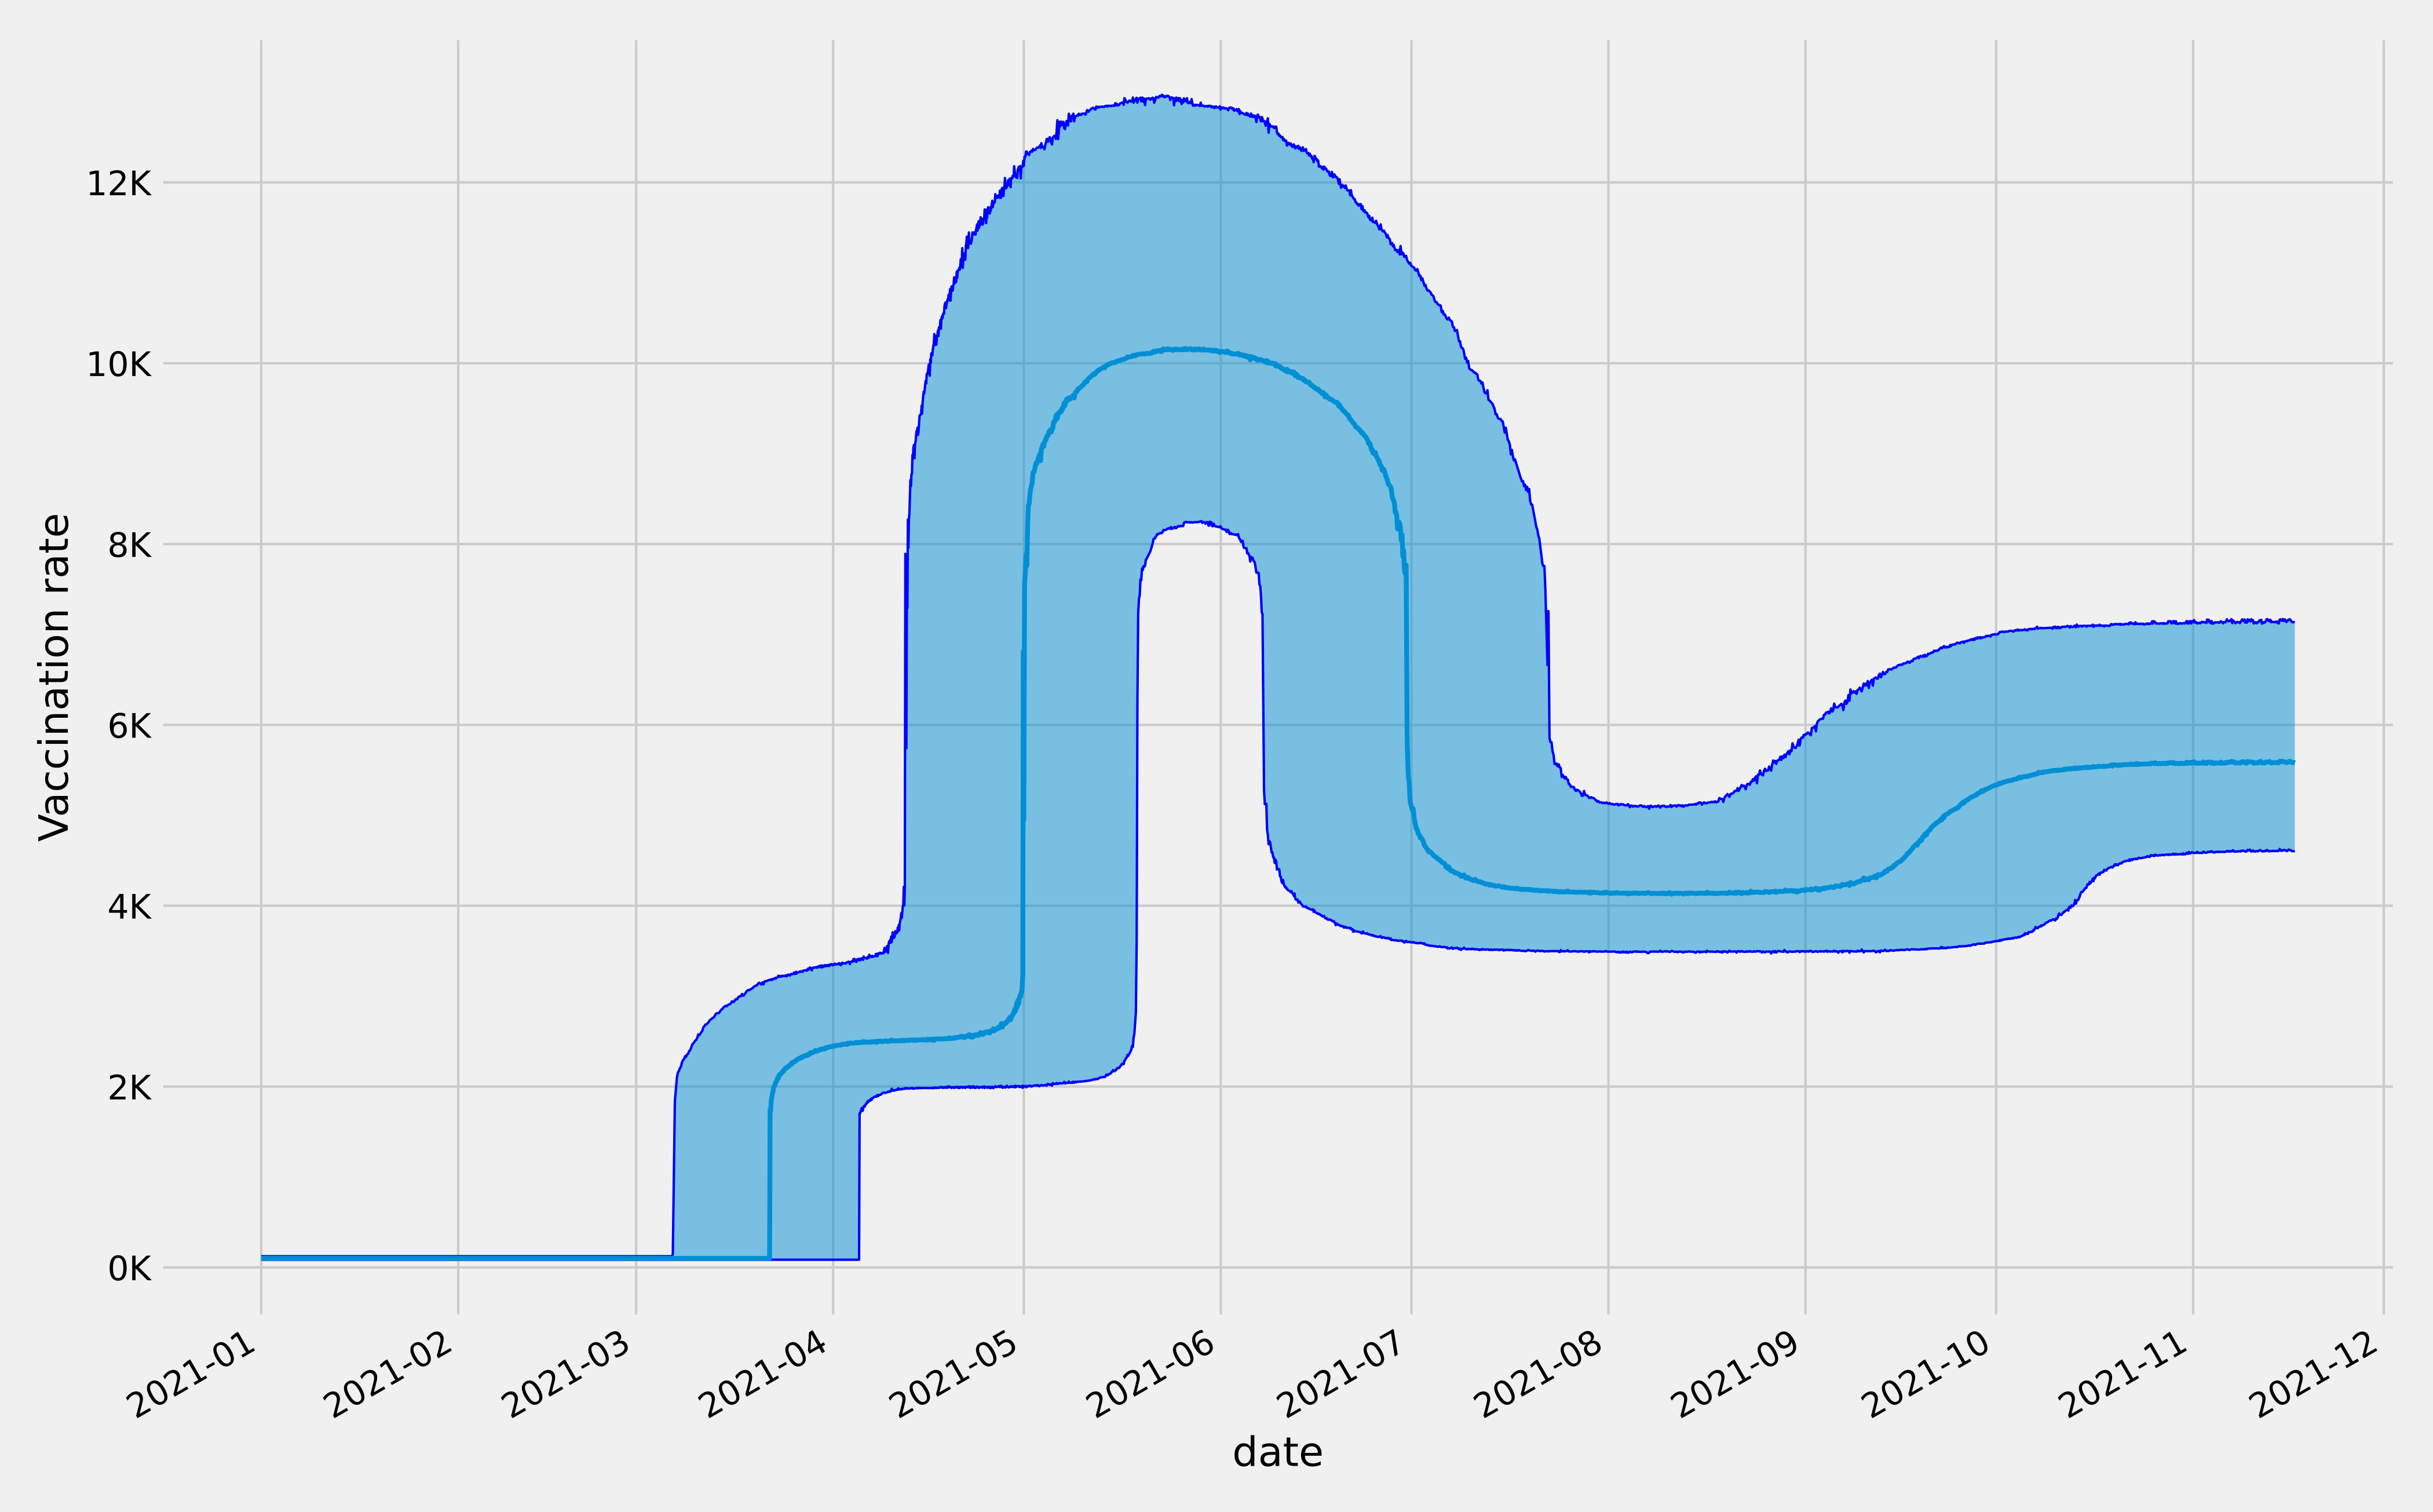
\includegraphics[width=1.05\linewidth]{assets/action.png}
\end{frame}
     \section{TODO list}
        \begin{frame}{TODO List}
    \begin{itemize}
        \item
            To describe fluctuations due to the uncertainty of vaccine immunity by
            a mean reversible process.
            $$
                d \Psi_V(t) =  r_k  (\Psi_V^{K} - \Psi_V(t)) dt + \sigma
                \sqrt{\Psi_V(t)} dW
            $$
        \item Propose a cost functional ( DALYs, Risk, $R_t$ )
        \item Optimize in a convenient space of actions.
        \item Partially observable models
        \item Stochastic GAMES
    \end{itemize}
\end{frame}

\begin{frame}{}
    \centering
    \Huge{GRACIAS!!}
    \\
    \normalsize
    \href{%
        https://github.com/SaulDiazInfante/
        Baemer-SIAM-Section-Mexico-third-annual-Metting.git}{
        Git Hub}
    \\
    \insertqrcode
\end{frame}
\end{document}
